\part{Modélisation du théâtre d’Orange} \label{part_1}

	\chapter*{Introduction}
	%\addcontentsline{toc}{chapter}{Introduction}
	 \addstarredchapter{Introduction} \label{introarcheo}
	 
			 Le théâtre antique d'Orange situé dans le Vaucluse est le théâtre romain le mieux conservé d'Europe et un des trois seuls au monde à avoir conservé son mur de scène. Il est adossé à la colline Saint-Eutrope sur laquelle sa \gls{cavea} repose partiellement.
			 
			 En 45 avant notre ère, suite à la victoire de César sur la Gaule, de larges vagues de colonisations amenèrent des soldats vétérans à s'installer dans la province de Gaule transalpine qu'Auguste réorganise par la suite en province de Narbonnaise. L'architecture urbaine est régie par certains préceptes dont les écrits de Vitruve \cite[Livre V]{vitruve} donnent un aperçu. De nombreux théâtres sont alors construits selon une structure assez semblable comme par exemple celui d'Arles bâtie en 20 avant notre ère. La construction du théâtre de Aurosio (l'ancienne ville d'Orange) fut démarrée par les vétérans de la II\up{e} légion gallique de César vers 10 avant notre ère et dura quelques dizaines d'années \cite[p. 31]{PouvoirDuTheatre}. Cette origine nous est d'ailleurs rappelée par la présence du sigle C.I.S (\textit{Colonia Iulia Secundanorum}) inscrit à plusieurs endroits du grand mur du \gls{postscaenium} \cite[p26]{formige}.
			 
			 Lorsque le théâtre fut abandonné comme édifice de spectacle, il ne fut pas détruit. Les princes d'Orange y firent installer un poste avancé de leur château et l’ensemble de l’édifice fut investi par des habitations utilisant le mur de scène comme rempart de protection (fig. \ref{av_deblaiement}). Au XVII\up{e} siècle le roi Louis XIV qualifiait en ces mots son impressionnant mur de scène de 103m de large par 37m de haut comme : « La plus belle muraille de mon royaume » et quelques écrits tentèrent déjà d'imaginer les démonstrations qui pouvaient se tenir dans ce lieu de spectacle. 
			 
			 Ce n'est pourtant qu'au XIX\up{e} siècle que débuta un vaste chantier de déblaiement de l'enceinte dans le but de restituer au bâtiment son rôle premier. Avec ce projet apparurent les premières images d'archive du théâtre. En charge du chantier, Augustin Caristie fait paraitre en 1846 \textit{"Monuments antiques à Orange, arc triomphe et théâtre"}, oeuvre de référence qui recense l'état des vestiges avant et après la destruction des maisons. Ces textes et dessins bien que, comme le stipule l'auteur, parfois hypothétiques sont par la suite complétés par d'autres architectes comme Pierre-Honoré Daumet qui réalisa en 1873 le relevé des élévations du monument. Les premières représentations théâtrales modernes purent alors avoir lieu. \`{A} la fin du siècle l'architecte Jean-Camille Formigé fut chargé de restaurer la \gls{cavea} selon les indications de A.Caristie et en s'inspirant du modèle de Vitruve. Son fils Jules Formigé poursuivit son travail et mis à jour de nombreux éléments de décors notamment en creusant au niveau de l'\gls{hyposcaenium}. Depuis les années 20 jusqu'aux années 80 de nombreuses restaurations ou constructions ont été effectuées avec une rigueur archéologique contestable dans le but principalement d'habiller le lieu plus que pour le restituer. En 1981, le théâtre entre au patrimoine mondiale de l'UNESCO et quelques années plus tard d'autres constructions modernes telle que la couverture métallique de la scène viennent s'ajouter, détériorant au passage une partie de la maçonnerie antique. Certains projets ont pu être stoppés avant que des dégâts irréparables ne soient créer comme la créations d'ascenseurs dans le mur de scène. Malgré tout, ces travaux ont souvent été entrepris sans le moindre regard archéologique et de nombreuses données ont été perdues \cite[p 231- 236]{carteArcheo}.

			 
			 Depuis la fin du XX\up{e} siècle l'\gls{iraa} a relancé une étude approfondie du bâtiment et de sa décoration avec une approche archéologique rigoureuse. Ce projet de thèse s'articule dans la continuité de cette étude avec pour objectif : la modélisation numérique du théâtre. La première partie de ce document présente l'agencement architectural du bâtiment sans entrer dans les détails de sa décoration. Elle est suivie par la description détaillée des méthodes de modélisation graphique ayant permis de créer le modèle numérique. Celui-ci compile une grande partie des informations architecturales du théâtre dans sa version d'origine. Nous expliquerons d'où proviennent ces diverses informations, quel crédit nous pouvons leur accorder et les problèmes soulevés par ce travail. Certaines hypothèses des architectes ayant étudié ce monument seront remise en question et d'autres seront explorées afin d'en déterminer la vraisemblance. Cette partie se terminera par la présentation de certaines applications et tests visuels élaborés à partir du modèle numérique.
			 
		
\begin{figureth}
	\begin{subfigureth}{0.49\textwidth}
		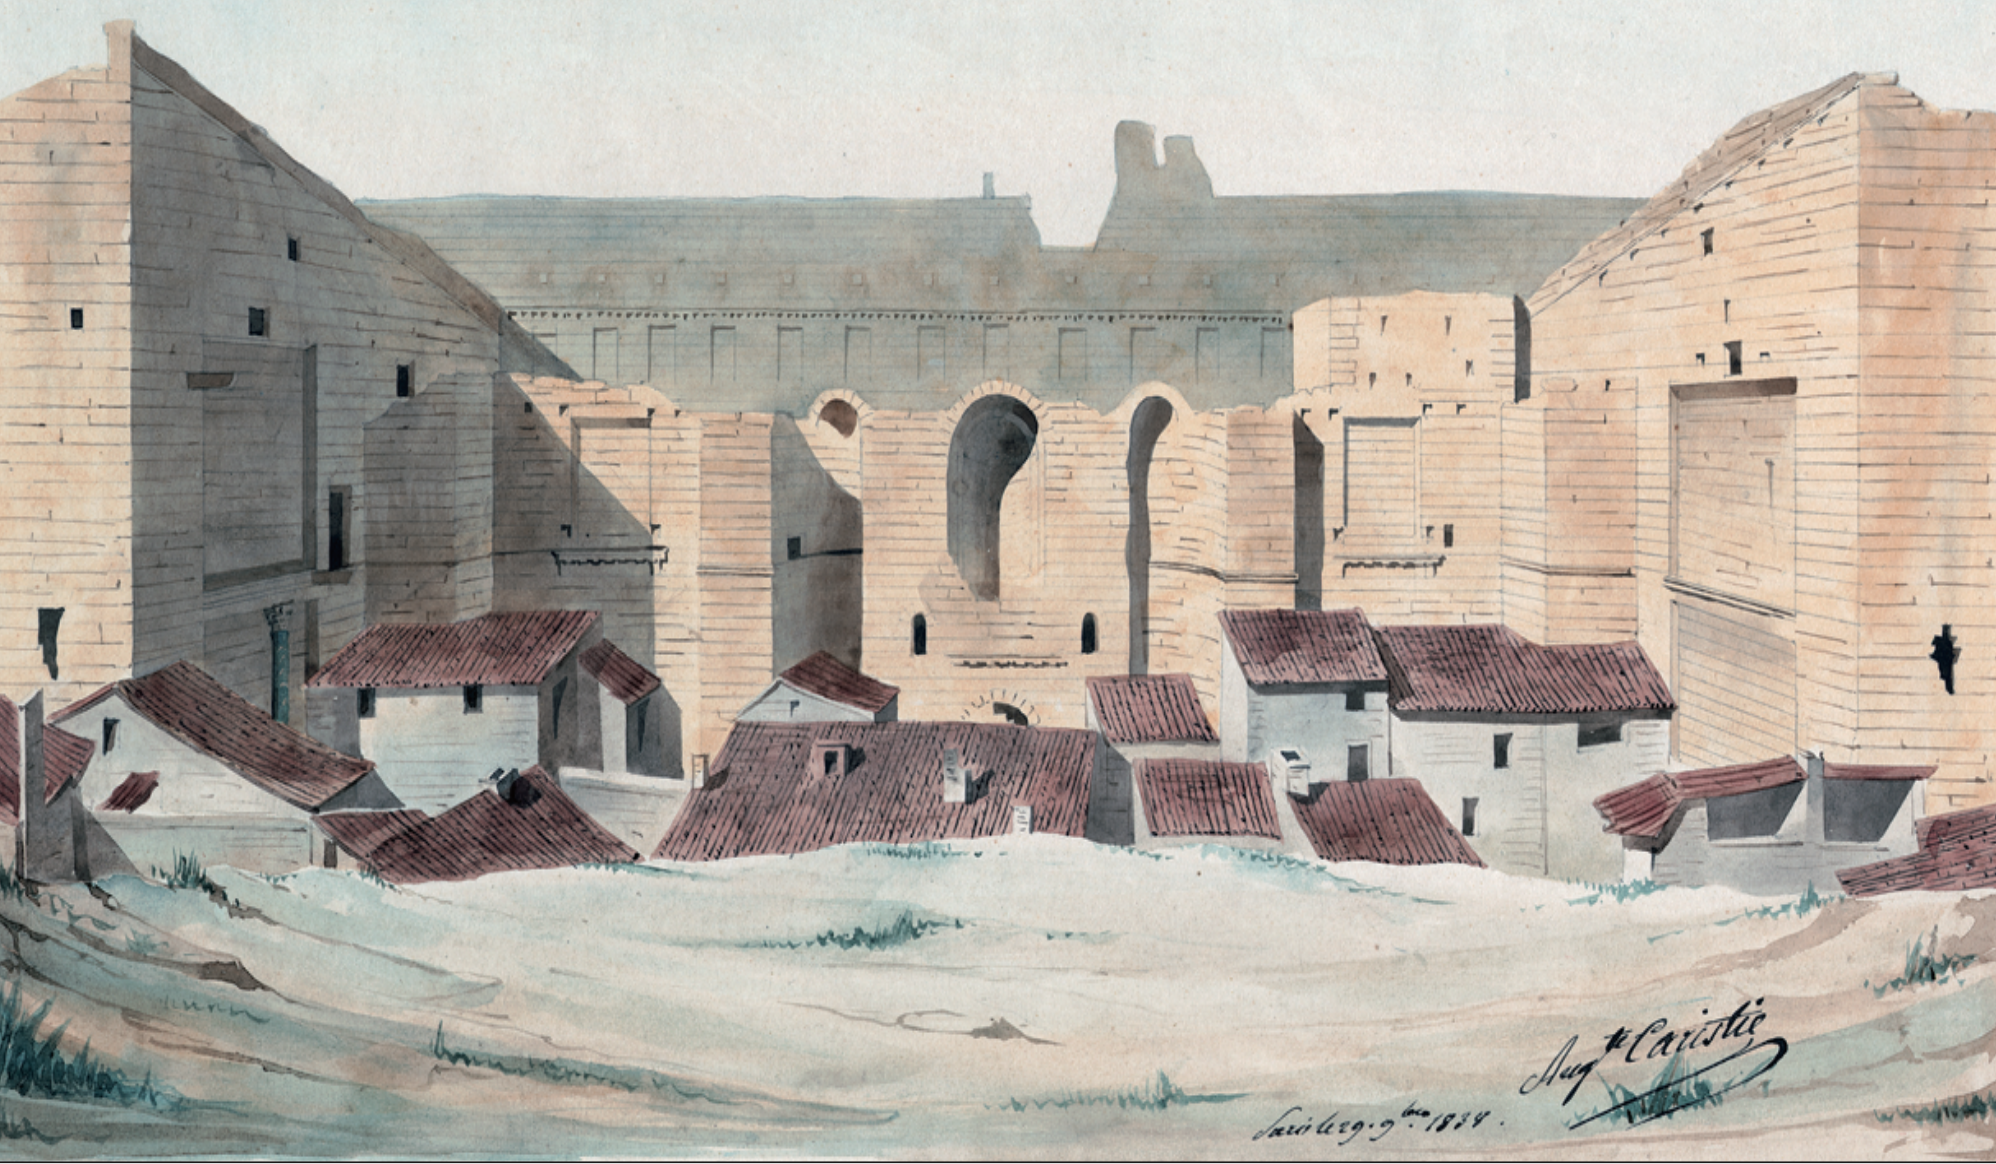
\includegraphics[width=\linewidth]{images/av_deblaiement}
		\caption{Vue de la scène avant le déblaiement par A. Caristie \footnotemark}
		\label{av_deblaiement}
	\end{subfigureth}
	\begin{subfigureth}{0.47\textwidth}
		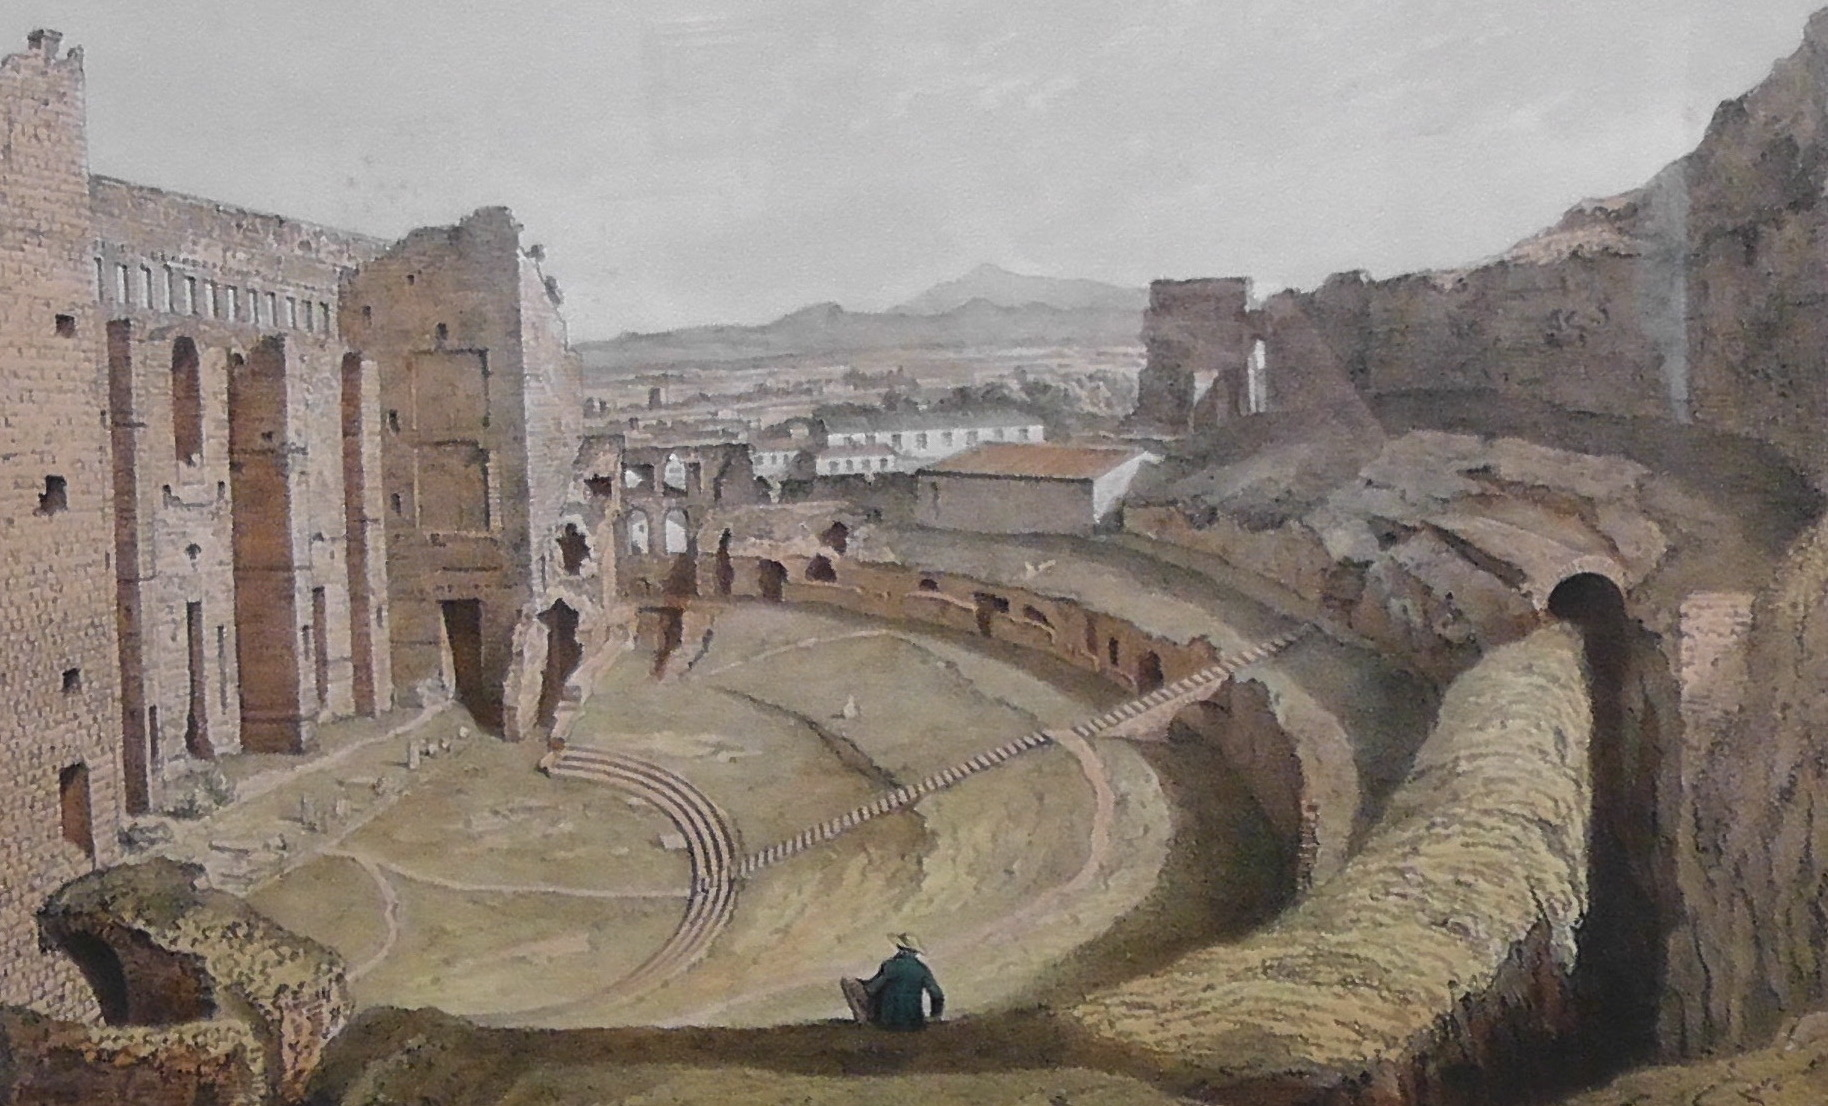
\includegraphics[width=\linewidth]{images/asselineau}
		\caption{Vue intérieure du théâtre par Asselineau \footnotemark}
	\end{subfigureth}
	\caption[Théâtre d'Orange avant restauration]{Dessins du théâtre d'Orange avant et après déblaiement par A.Caristie}		
	%\label{fig:caristie}
\end{figureth}		
\addtocounter{footnote}{-1}
\citefnt[cliché]{charenton}
\addtocounter{footnote}{1}
\citefnt[cliché]{museeOrange}
		
	\chapter{Présentation synthétique de l'architecture du théâtre d'Orange}
		\citationChap{
		L'architecture, c'est ce qui fait les belles ruines
		}{Auguste Perret}
		\minitoc
		\newpage
		
		\section{Introduction}
		
		En 2013, l'\gls{iraa} conclue une série de campagnes de relevés et d'analyse du théâtre d'Orange démarrée en 1998. Ce travail recense les relevés effectués sur le terrain ainsi qu'une étude approfondie des documents d'archive, conservés pour la plupart à la Médiathèque de l'architecture et du patrimoine à Charenton-le-Pont. Ceux-ci comportent les plans des architectes A.Caristie et P.G.H.Daumet et permettent d'avoir un état des lieux du théâtre avant que celui-ci ne soit restauré par J.Formigé. L'étude réalisée durant cette thèse est donc principalement basée sur le rapport de l'\gls{iraa} résultant de ces travaux d'analyse \cite{orangeTxt}\cite{orangePl}.
		
		Le théâtre d'Orange a été bâti en grande partie selon préceptes de l'architecture romaine de l'époque impériale. Comme la plupart de ces édifices, il se présente en demi-cercle fermé par un mur rectiligne. Sa \gls{cavea} tournée vers le nord est adossée à la colline Saint-Eutrope qui offre un support naturel à l'édifice. A la différence des \glspl{odeon} qui étaient entièrement couverts, seul un \gls{velum} couvrait l'espace réservé aux spectateurs. Collées au flan est du théâtre se trouvent les ruines d'un sanctuaire du culte impérial qui ne fait pas partie de l'étude. De même, la façade nord était prolongée par une grande \gls{porticus ps} qui n'a pas été modélisée mais qui pourra l'être dans une étude postérieure. 
		
		Ce chapitre présente l'architecture non détaillée du théâtre d'Orange par grands sous-ensembles. Il servira d'introduction au chapitre suivant et permettra au lecteur de se familiariser avec le monument en le replaçant dans son contexte d'utilisation.

	\begin{figureth}
			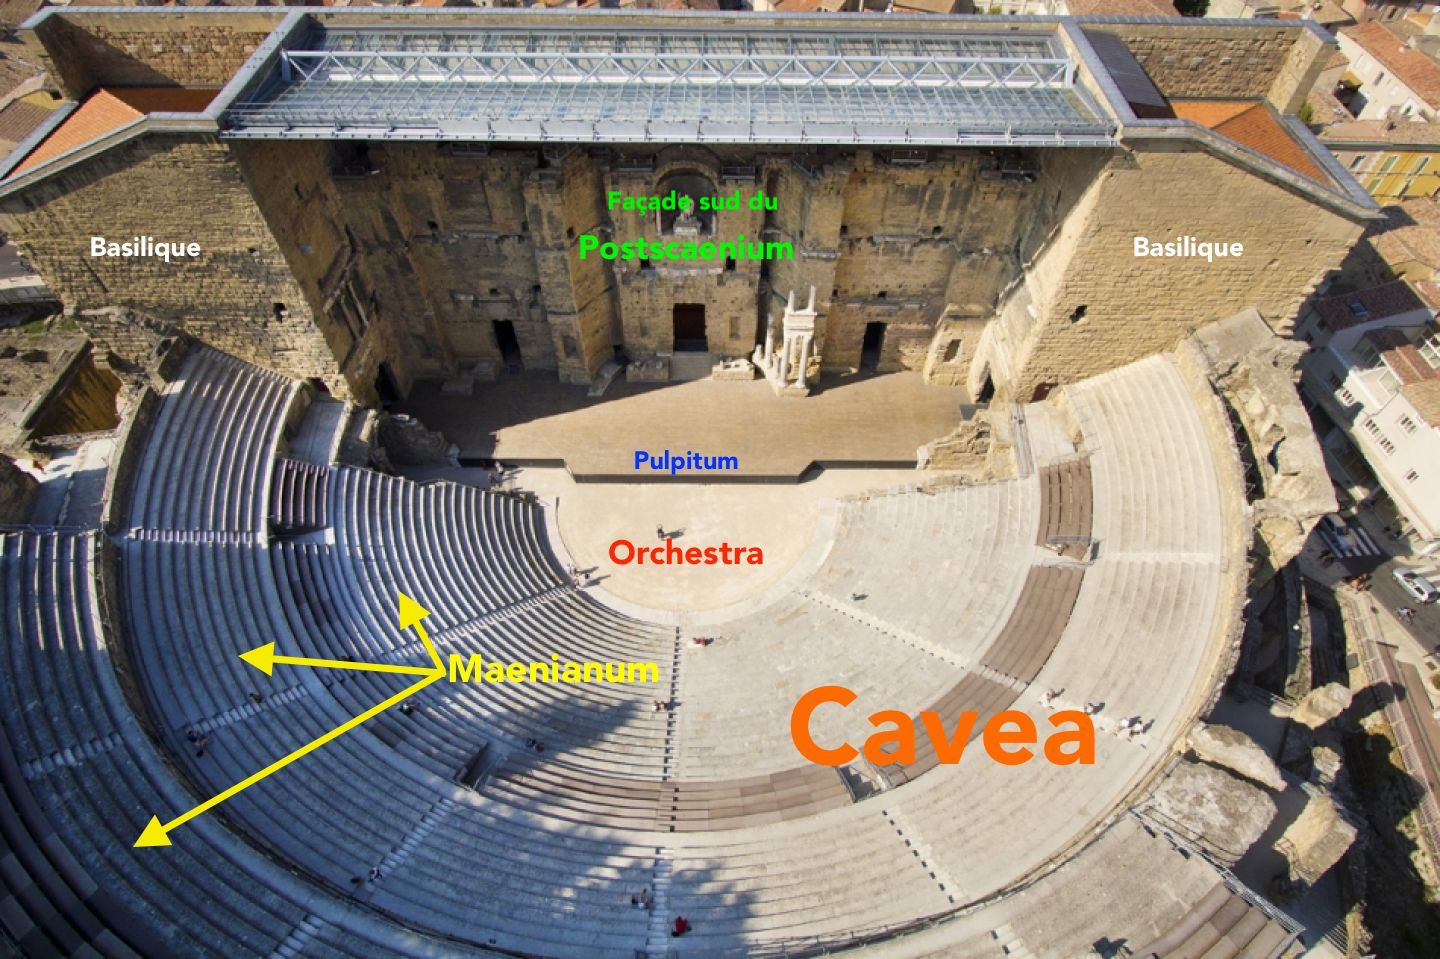
\includegraphics[width=\linewidth]{images/vuensemble}
			\caption[Vue d'ensemble du théâtre d'Orange]{Vue d'ensemble du théâtre d'Orange \footnotemark}
	\end{figureth}
\citefnt[cliché]{vuEnsemble}

\section{Le \gls{postscaenium}, les \glspl{basilique} et le \gls{pulpitum}}
\label{sect_postscaenium}
		
		Le \gls{postscaenium} (ou mur de scène) constituant la façade nord du bâtiment, ainsi que les deux \glspl{basilique} l'enclavant, constituent les parties les mieux conservées du théâtre. Le \gls{postscaenium} servait de décor pour les représentations et tenait probablement un rôle acoustique (voir \autoref{part3}). Les côtés est et ouest donnaient sur des rues, alors qu'adossée à la façade nord se trouvait une \gls{porticus ps} large d'environ neuf mètres. Celle-ci donnait accès au \gls{postscaenium} par le biais de dix-sept portes reparties de manière symétrique de part et d'autre de la porte centrale. Le deuxième niveau du mur est orné, dans sa partie haute, d'une série d'arcades composée de vingt-deux \glspl{pilastre}. Au troisième niveau de la façade se trouvent deux séries de \glspl{console} ainsi qu'une assise de bouches d'eau qui permettaient d'évacuer les eaux qui tombaient sur le toit du bâtiment de scène. Les \glspl{console} de la série supérieure présentent un trou traversant permettant d'accueillir les mâts de maintient du \gls{velum}. Seules les deux \glspl{console} situées aux extrémités font exeption. Celles de la série inférieure sont creusées à leur lit d'attente d'une grande mortaise circulaire prolongée par un petit trou permettant l'écoulement de l'eau de pluie. Pour pouvoir placer un mât dans un couple de \glspl{console}, il fallait également que l'assise de bouche d'eau soit percée. Or cela n'est le cas que pour douze emplacements correspondant aux mâts \no4 à 9 à partir des deux extrémités du mur. Il semble donc que les mâts n'aient été présents qu'à ces emplacements, c'est à dire au niveau des \glspl{basilique}. L'absence de mât au niveau du mur de scène pourrait s'expliquer par le fait que la forte tension liée au poids du \gls{velum} aurait été trop importante pour un mur rectiligne de cette longueur et cette épaisseur. La forme carrée des basiliques permet une plus grande résistance à la tension. Néanmoins, il est aussi possible de supposer que les \glspl{console} aient été initialement prévues pour couvrir l'estrade par des voiles montées sur des vergues comme à Aspendos et que l'idée fut abandonnée en cours de construction au profit d'une toiture de tuiles sur charpente de bois \cite[p. 144-147]{moretti}. 
		
		Le \gls{postscaenium} comporte huit pièces donnant uniquement sur la \gls{porticus ps} à l'extérieur du théâtre. Ces pièces servaient de coulisses pour l'habillement des acteurs ou le stockage des décors et des costumes \cite[p. 56]{formige}. Trois portes, dont la porte royale, donnent directement accès à la scène. Deux portes de part et d'autre conduisent aux \glspl{basilique} et une à des escaliers permettant de monter aux étages supérieurs via les \glspl{parascaenium}. \`{A} l'intérieur du \gls{postscaenium}, en plus du rez-de-chaussée et des combles, on compte deux étages assurés par la présence de baies à arcatures permettant de passer d'une pièce à l'autre. Cela permettait aux acteurs d'accéder à des niches traversantes en hauteur pour faire apparaitre sur le front de scène des personnages divins (ou effectuer des bruits de tonnerre par exemple).
		
		La façade sud du mur (ou front de scène) est celle qui servait de décor aux spectacles. Aujourd'hui, il ne reste que le mur en calcaire de Courthézon (calcaire de couleur jaune foncé-beige) qui été jadis partiellement caché par des ornementations en marbre. On y trouve plusieurs niches de diverses profondeurs ainsi que les traces d'encastrement du placage de marbre qui servent aujourd'hui de repère aux archéologues pour reconstituer la décoration. Le mur a une géométrie quasi-symétrique par rapport à l'axe décrit par la porte royale rectangulaire et la niche voutée, située au dessus, accueillant aujourd'hui une statue dite "d'Auguste" (faite de ciment et de fragments antiques et placée là en 1944). Cet axe est placé sur une paroi rectiligne qui fait saillie au fond d'une \gls{exedre} curviligne ce qui attire naturellement l'oeil vers la porte royale et la niche voutée. De part et d'autre se trouvent deux \glspl{exedre} rectangulaires peu profondes. Le mur est divisé verticalement en trois ordres sur les extrémités et seulement deux sur la partie centrale. Au dessus de façade se trouve l'espace réservé au toit qui couvrait le \gls{postscaenium} et la scène. On y voit aujourd'hui les trous d'encastrement dans lesquels venaient s'insérer les poutres.
		
		Le mur de façade du bâtiment de scène est flanqué de part et d'autres de deux \glspl{basilique} de forme presque carrée auxquelles on accède depuis la scène en traversant un \gls{parascaenium}. Celui-ci communique avec la basilique via une porte arquée et à la scène par une une grande porte rectangulaire. \gls{parascaenium} comporte une cage d'escaliers permettant d'atteindre les niveaux supérieurs du \gls{postscaenium}. Les \glspl{basilique} sont composées de deux niveaux séparés par un plancher en bois et accessible que depuis le rez-de-chaussée. On retrouve cela dans les théâtres d'Arles, Aspendos ou de Marcellus à Rome par exemple \cite[p. 35]{formige}. Leur taille monumentale semble indiquer une fonction de foyer luxueux permettant aux spectateurs de se retrouver pendant les entre-actes ou en cas d'intempéries. Elles pouvaient également servir de coulisses pendant les spectacles ou pour stocker les éléments de décor volumineux. Ces salles étaient accessibles par les trois cotés autres que la scène par un couple de baies à arcature. 
				
		La scène ou \gls{pulpitum} était une structure en bois d'une largeur de 61m et d'une profondeur de 10m qui a complètement disparu. Sa façade était ornée par une décoration de marbre souvent composée de niches rondes ou carrées alternées. Vitruve \cite[p. 10-11]{vitruve} dit que sa largeur doit valoir le double du diamètre de l'orchestre et que sa hauteur ne doit pas excéder cinq pieds (soit 1m50) afin que les spectateurs assis dans l'orchestre voient facilement. Celle de Orange s'élève à 1m25 d'après les traces laissées sur le mur de scène \cite[p. 318-319]{orangeTxt}. Le mur de façade ornant le \gls{pulpitum} est défini du côté de l'orchestre par un caniveau et de l'autre côté par l'alignement avec des cassettes. J.Formigé en mesure ainsi une épaisseur de 75cm supposant qu'il n'était pas orné de niches mais plutôt d'une frise continue comme au théâtre de Dionysos à Athènes \cite[p. 457]{formigeBis}. En dessous se trouve l'\gls{hyposcaenium} qui étaient composé principalement d'une fosse et d'un espace dédié à la machinerie du rideau de scène. En effet, entre le mur de front du \gls{pulpitum} et la scène, un rideau en étoffe peinte ou tissée d'une hauteur de moins de trois mètres descendait pour laisser apparaitre la scène aux spectateurs. Il venait s'enrouler autour de cylindres et était actionné par un système de poulies et contrepoids. Lorsque le rideau était descendu, le plancher venait fermer cet espace permettant ainsi aux acteurs de s'approcher jusqu'au bord du \gls{pulpitum}, voire de descendre au niveau de l'\gls{orchestra}. Le plancher était soutenu par des poutres et les acteurs ou les machinistes pouvaient se rendre en dessous par le biais de trappes et d'escaliers. La présence d'escaliers menant de la scène à l'orchestre n'est pas prouvée, néanmoins, deux escaliers de quatre marches étaient présents aux extrémités du \gls{pulpitum} et permettaient d'accéder aux \glspl{parodos} \cite[p. 458]{formigeBis}.
		
	\begin{figureth}
		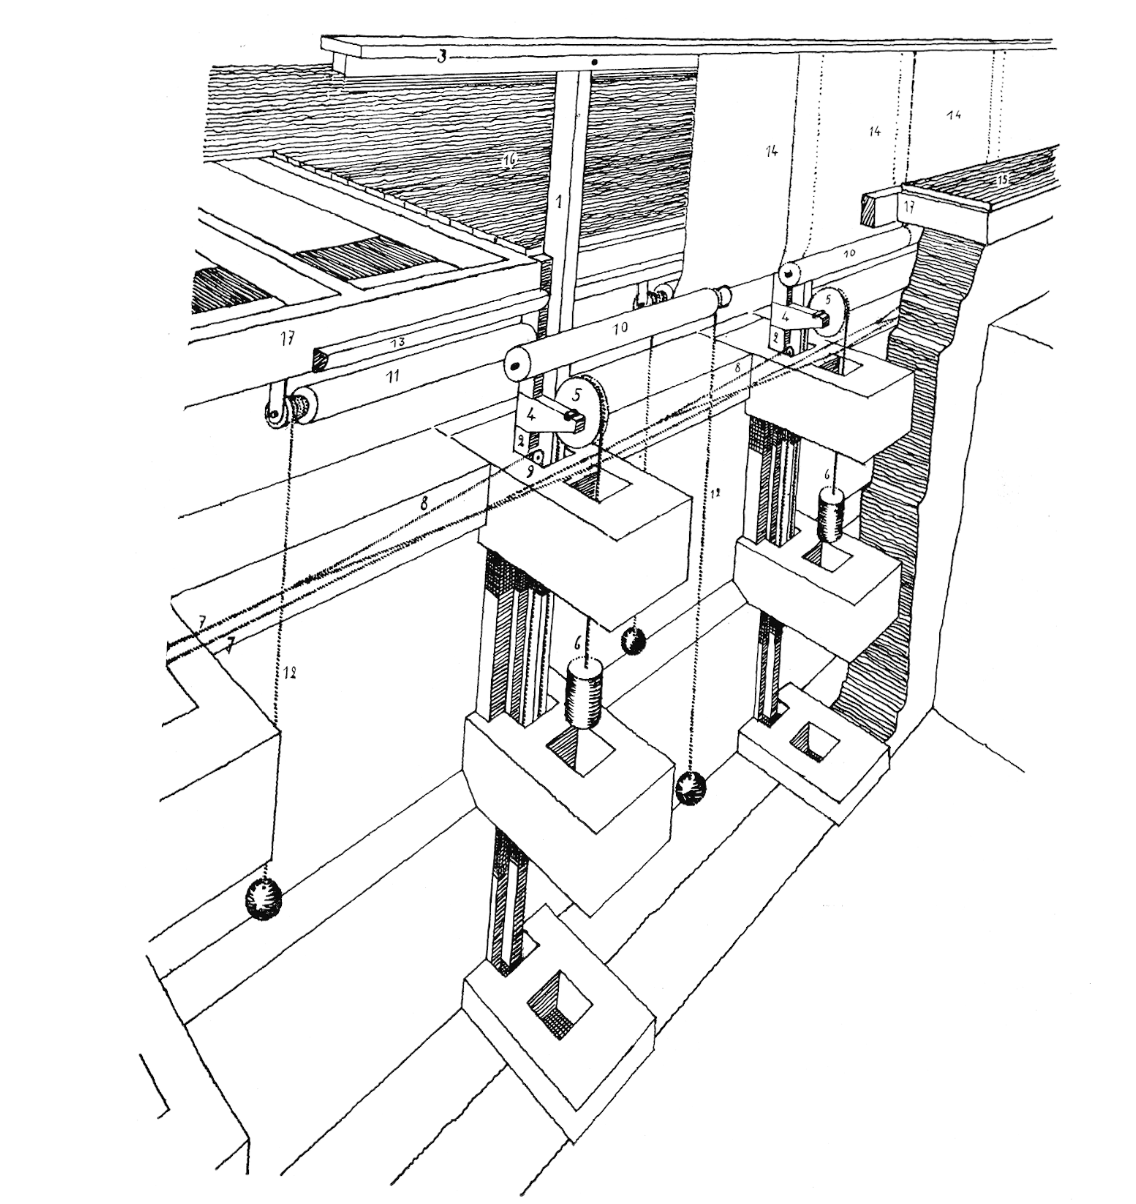
\includegraphics[width=0.6\linewidth]{images/rideau}
		\caption[Perspective d’une section de la fosse du rideau de scène au théâtre de Lyon]{Perspective d’une section de la fosse du rideau de scène au théâtre de Lyon et restitution de la machinerie \footnotemark}
	\end{figureth}
\citefnt[fig. 11, p. 70]{rideau2}
						
		
\section{L'\gls{orchestra}, les \glspl{aditus} et la \gls{cavea}}		
	
	L'\gls{orchestra} est la partie semi-circulaire située entre la scène et le premier gradin. Anciennement nommée "choros" chez les grecs où elle accueillait le choeur, elle ne servirait plus aux représentations chez les romains d'après Vitruve \cite[p. 10]{vitruve} : "\textit{l'orchestre est réservé pour les sièges des sénateurs}. Cependant, Formigé \cite[p. 28-29]{formige} conteste cette hypothèse en affirmant que : "\textit{si l'on examine avec attention un orchestre romain, on remarque de suite qu'il se divise en deux parties : l'une, horizontale, souvent dallée de marbres rares comme à Arles, à Athènes, à Carthage, à Pompéi, etc., ou même de mosaïques comme à Chemtou; l'autre, composée d'un ou de plusieurs gradins de pierre, larges et bas}. Il appuie ses dires sur une citation de Gaston Boissier \cite[article MIMVS]{boissier} stipulant que les mimes jouaient "\textit{in plano orchestra}". Cela lui permet de conclure que : "\textit{il y a bien une partie plane, libre, dans l'orchestre, et qu'elle ne comprend pas tout l'orchestre}. Il relève d'ailleurs des marques laissant supposé qu'il y aurait eu trois gradin d'une largeur de un mètre permettant d'accueillir des siège mobile pour les sénateurs \cite[p. 455]{formigeBis}. L'\gls{orchestra} est aujourd'hui recouverte de graviers compacts qui camoufle son aspect antique. Elle était limitée par un \gls{balteus} qui marquait la séparation avec la \gls{cavea} et qui surplombait un petit caniveau permettant d'évacuer l'eau de pluie. Elle comportait aussi des escaliers qui pouvaient mener à la scène soit par le centre soit par les extrémités \citep[p. 52]{formige}.
	
	Depuis l'extérieur du théâtre on accède à ce lieu par deux larges \gls{parodos} formant les \glspl{aditus}. Chacun est composé d'une succession de trois voûtes en décrochement qui portaient les extrémités de la \gls{cavea} et les tribunes. Ces dernières, considérées comme des places d'honneur, étaient souvent décorées de sculpture comme à Dougga ou à Herculanum et étaient accessibles par des escaliers particuliers \citep[p. 37]{formige}. Ces entrées étaient dallées sur toute leur longueur mais sont aujourd'hui recouvertes par un sol moderne \cite[Pl. XVI]{orangePl}.
	
		La  \gls{cavea}, telle qu'elle a été restaurée, comprend trois hémicycles appelés \glspl{maenianum}, séparés l'un de l'autre par une \gls{precinction} et un \gls{podium}. Cela a été déduit par A.Caristie grâce au profil des \glspl{aditus} et aux vestiges des substructures. C'est donc en ce sens que la \gls{cavea} fut reconstruite par Formigé. Chaque \gls{maenianum} est divisé par des escaliers en un certains nombre de sections appelées \glspl{cuneus}.
		
		Le premier \gls{maenianum}, ou \gls{ima cavea} est séparé par cinq escaliers en quatre \glspl{cuneus} comme le révèlent les vestiges des premiers gradins dégagés pendant les fouilles. Il comprend un repose-pied à sa base et vingt gradins comme à Aspendos, à Athènes (odéon d'Hérode Atticus) ou à Pompéi (grand théâtre) \citep[p. 34]{formige}. Leur hauteur moyenne est de 40cm et leur largeur de 80cm \cite[p. 31]{formige}. Au niveau de la première \gls{precinction}, neuf ouvertures donnent  sur un couloir souterrain (premier \gls{ambulacre}). Ce dernier est accessible depuis l'extérieur du théâtre au rez-de-chaussée par deux escaliers longeant les \glspl{aditus}. Le couloir ouvre aussi sur dix-huit pièces aveugles, mais seules les salles numérotées de 1 à 8 (fig. \ref{1erniveau}) sont des constructions antiques. Il était également possible de rejoindre le premier \gls{maenianum} à mi-hauteur depuis les \glspl{parodos} par le biais de deux escaliers installés sous les gradins. Ceux-ci n'ont pas été remis en fonction lors de la restauration. Les \glspl{vomitorium} et les \glspl{precinction} étaient généralement bordés de balustrades souvent ornées de sculptures.
		
	\begin{figureth}
		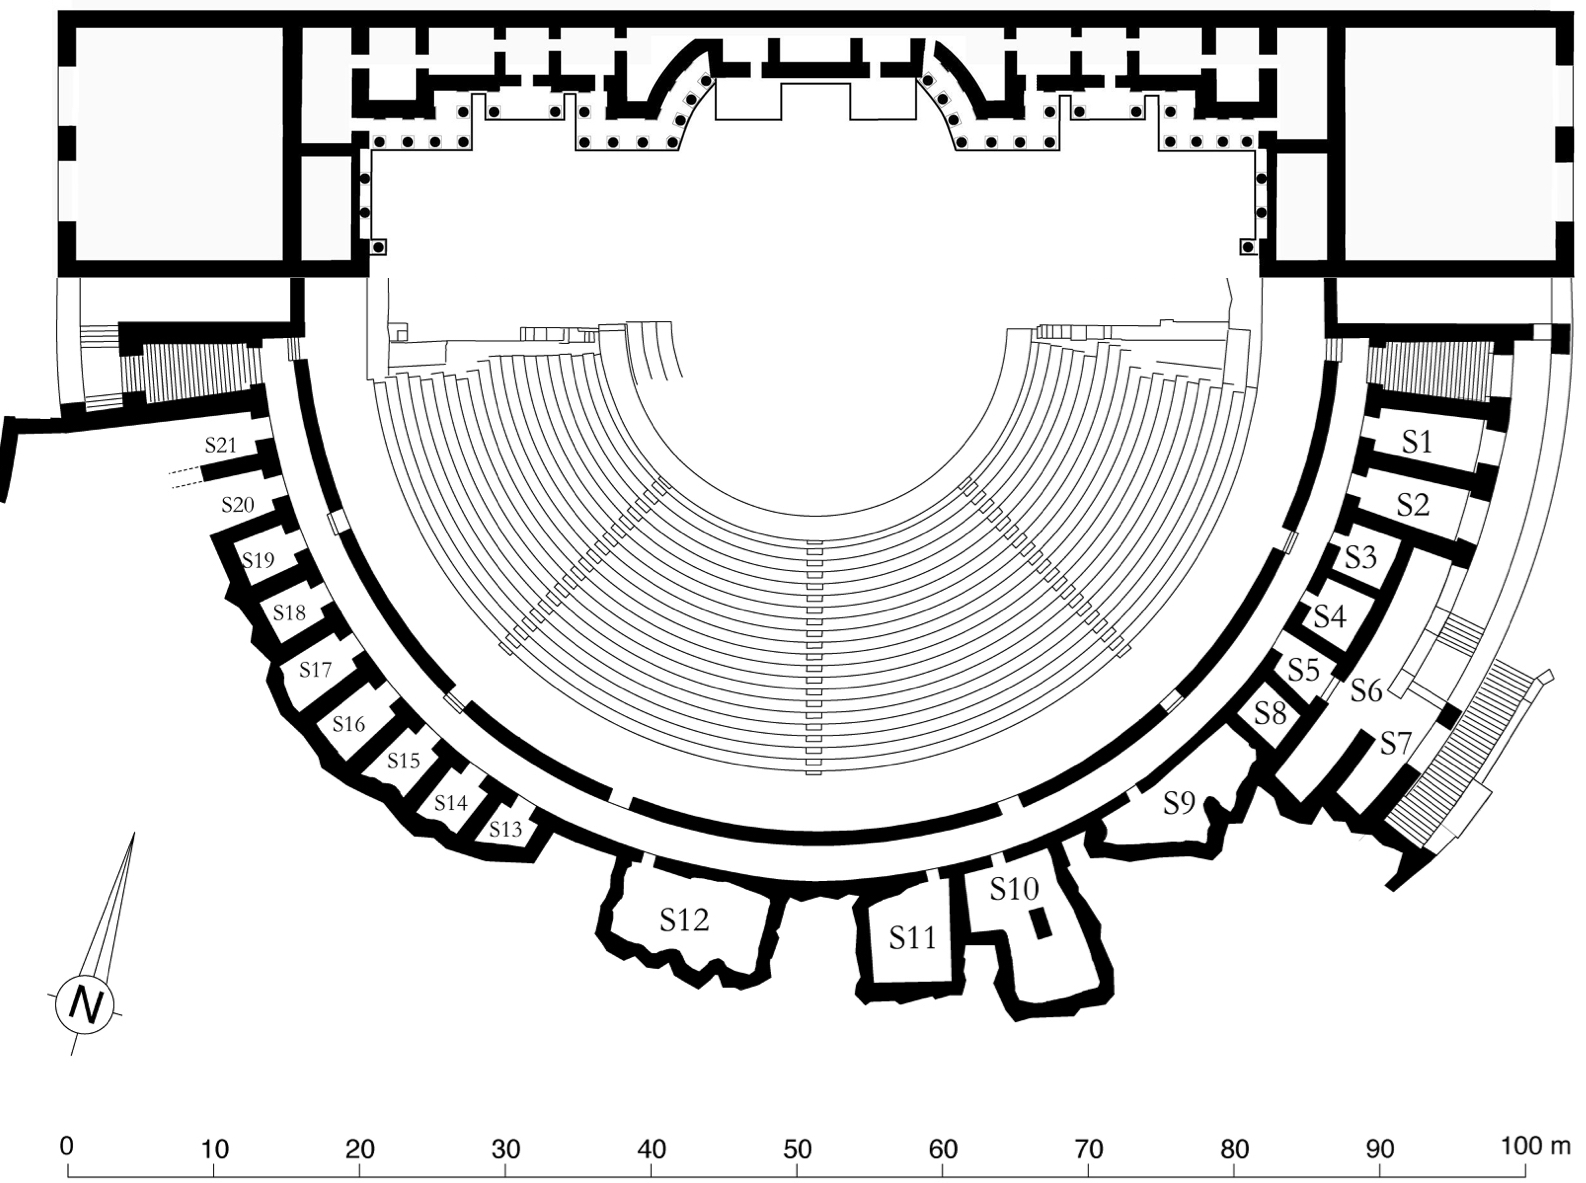
\includegraphics[width=\linewidth]{images/1erniveau}
		\caption[Vue de dessus - 1er niveau]{Plan du théâtre au niveau du premier \gls{ambulacre} \footnotemark }
		\label{1erniveau}
	\end{figureth}		
	\citefnt[Pl. XVII et XX fusionnées]{orangePl}
	
		
		Le deuxième \gls{maenianum}, ou \gls{media cavea}, repose, dans sa partie inférieure, sur l'\gls{ambulacre} du premier niveau et, dans sa partie supérieure, sur de la terre ou du remblai que complète, à proximité des \glspl{aditus}, deux niveaux de chambres voûtées. Il a été restauré pour former neuf gradins divisés en huit \glspl{cuneus} par neuf escaliers, ce qui semble être un choix acceptable en comparaison aux autres bâtiments du même type. Par ailleurs A.Caristie a relevé l'existence de cinq caissons de soutènement (C7 à C11 - fig. \ref{2emeniveau}) situés sous l'\gls{ima cavea} qui délimitent les passages permettant de se rendre au second \gls{ambulacre}. Celui-ci est souterrain dans la zone où la \gls{cavea} est adossée à la colline et construit sur deux niveaux de chambres voûtées dans sa partie la plus orientale. Il est directement accessible de l'extérieur par une porte à l'est et une autre à l'ouest.
		
	\begin{figureth}
		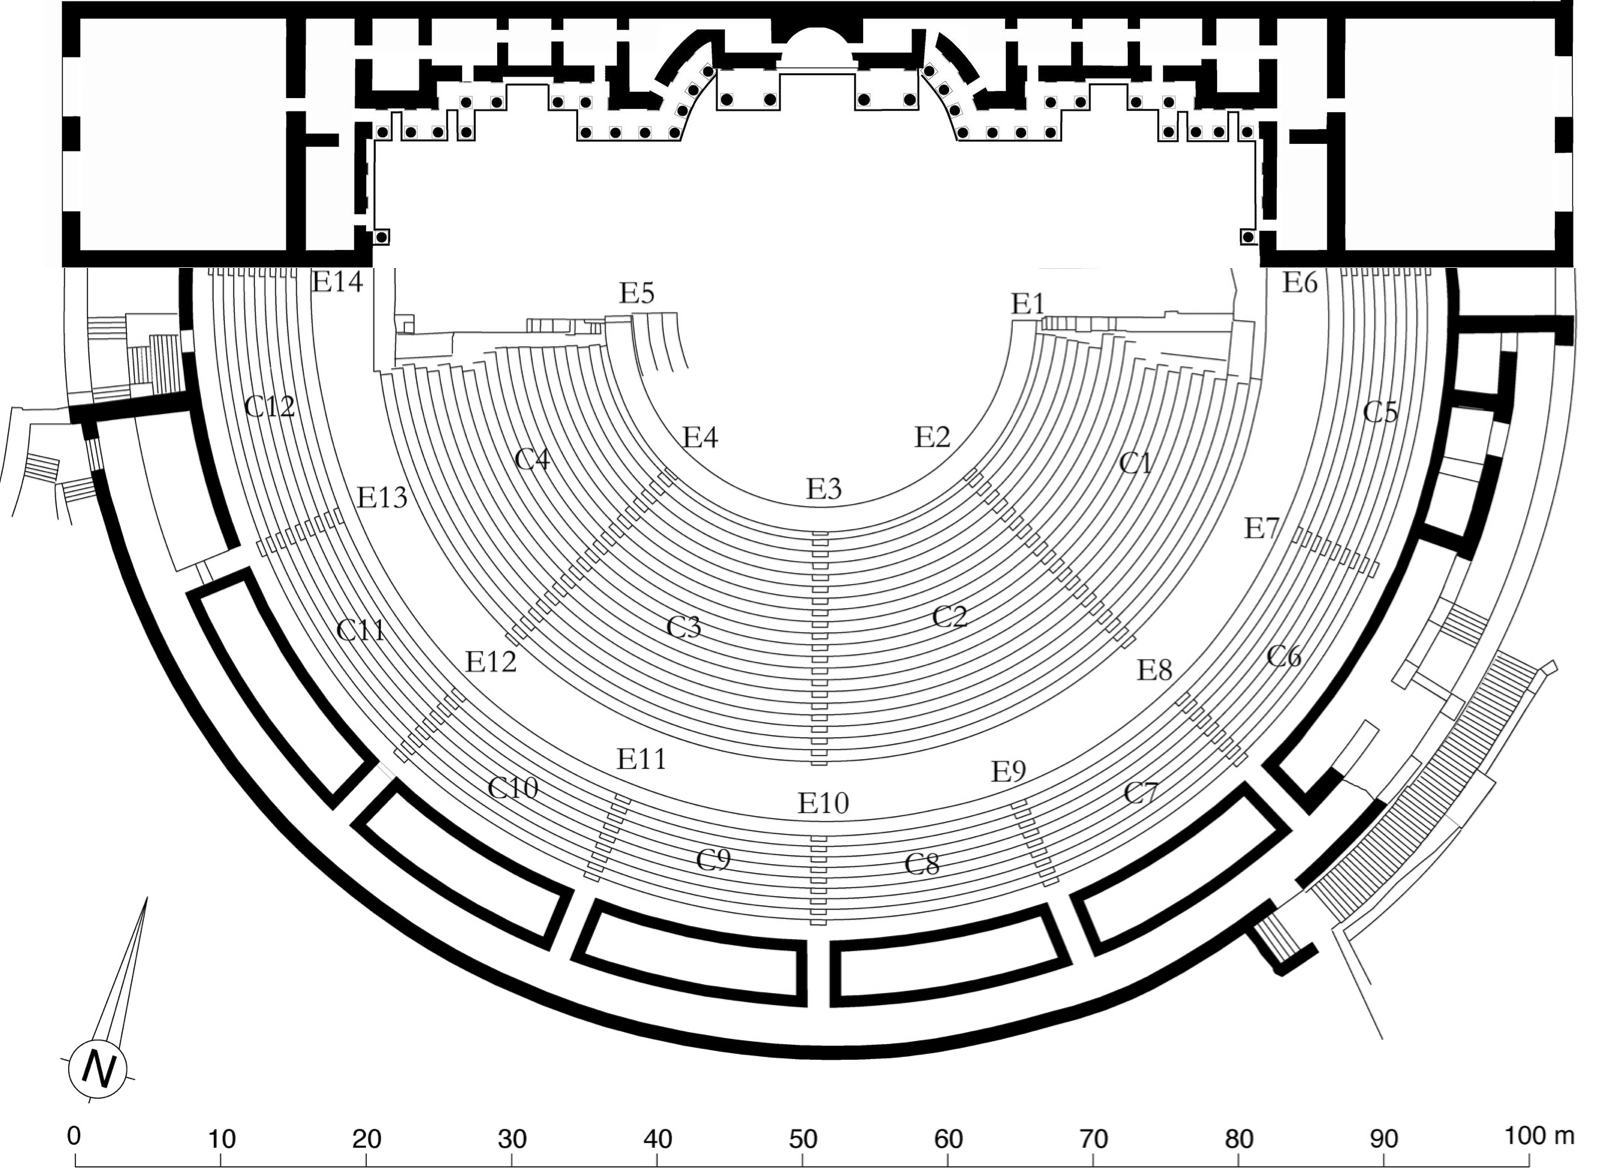
\includegraphics[width=\linewidth]{images/2emeniveau}
		\caption[Vue de dessus - 2ème niveau]{Plan du théâtre au niveau du second \gls{ambulacre} \footnotemark }
		\label{2emeniveau}
	\end{figureth}		
	\citefnt[Pl. XVIII et XX fusionnées]{orangePl}
		
		Le troisième \gls{maenianum}, ou \gls{summa cavea}, comporte cinq gradins divisés également par neuf escaliers. On constate que la largeur des gradins diminue lorsqu'on s'élève, ainsi, ils ne mesurent plus que 72cm en moyenne sur le troisième \gls{maenianum}, ce qui a pour effet d'augmenter la pente et d'améliorer la visibilité des derniers rangs. Il était jadis couronné par une \gls{porticus isc}, dont l'existence est assurée par des traces sur les faces méridionales des murs des \glspl{basilique}. D'une largeur de 3m55, il semble comporter un toit-terrasse donnant accès aux mécanismes \gls{velum}. On trouve aujourd'hui des gradins sur échafaudages à cet emplacement de même que sur les deux premières \glspl{precinction}. Une rue périphérique enclave la \gls{porticus isc} séparée par un mur que J-C.Formigé avait percé de quatre portes au niveau des escaliers E9 à E12 (fig. \ref{2emeniveau} et \ref{3emeniveau}). L'accès en face de E9 est probable, non seulement parce qu'H.Daumet a noté une interruption du mur périphérique à cet endroit \cite[Pl. VII]{orangePl}, mais aussi parce que le mur bordant la rue en amont est également percé d'une porte dans la prolongation de E9.


	\begin{figureth}
		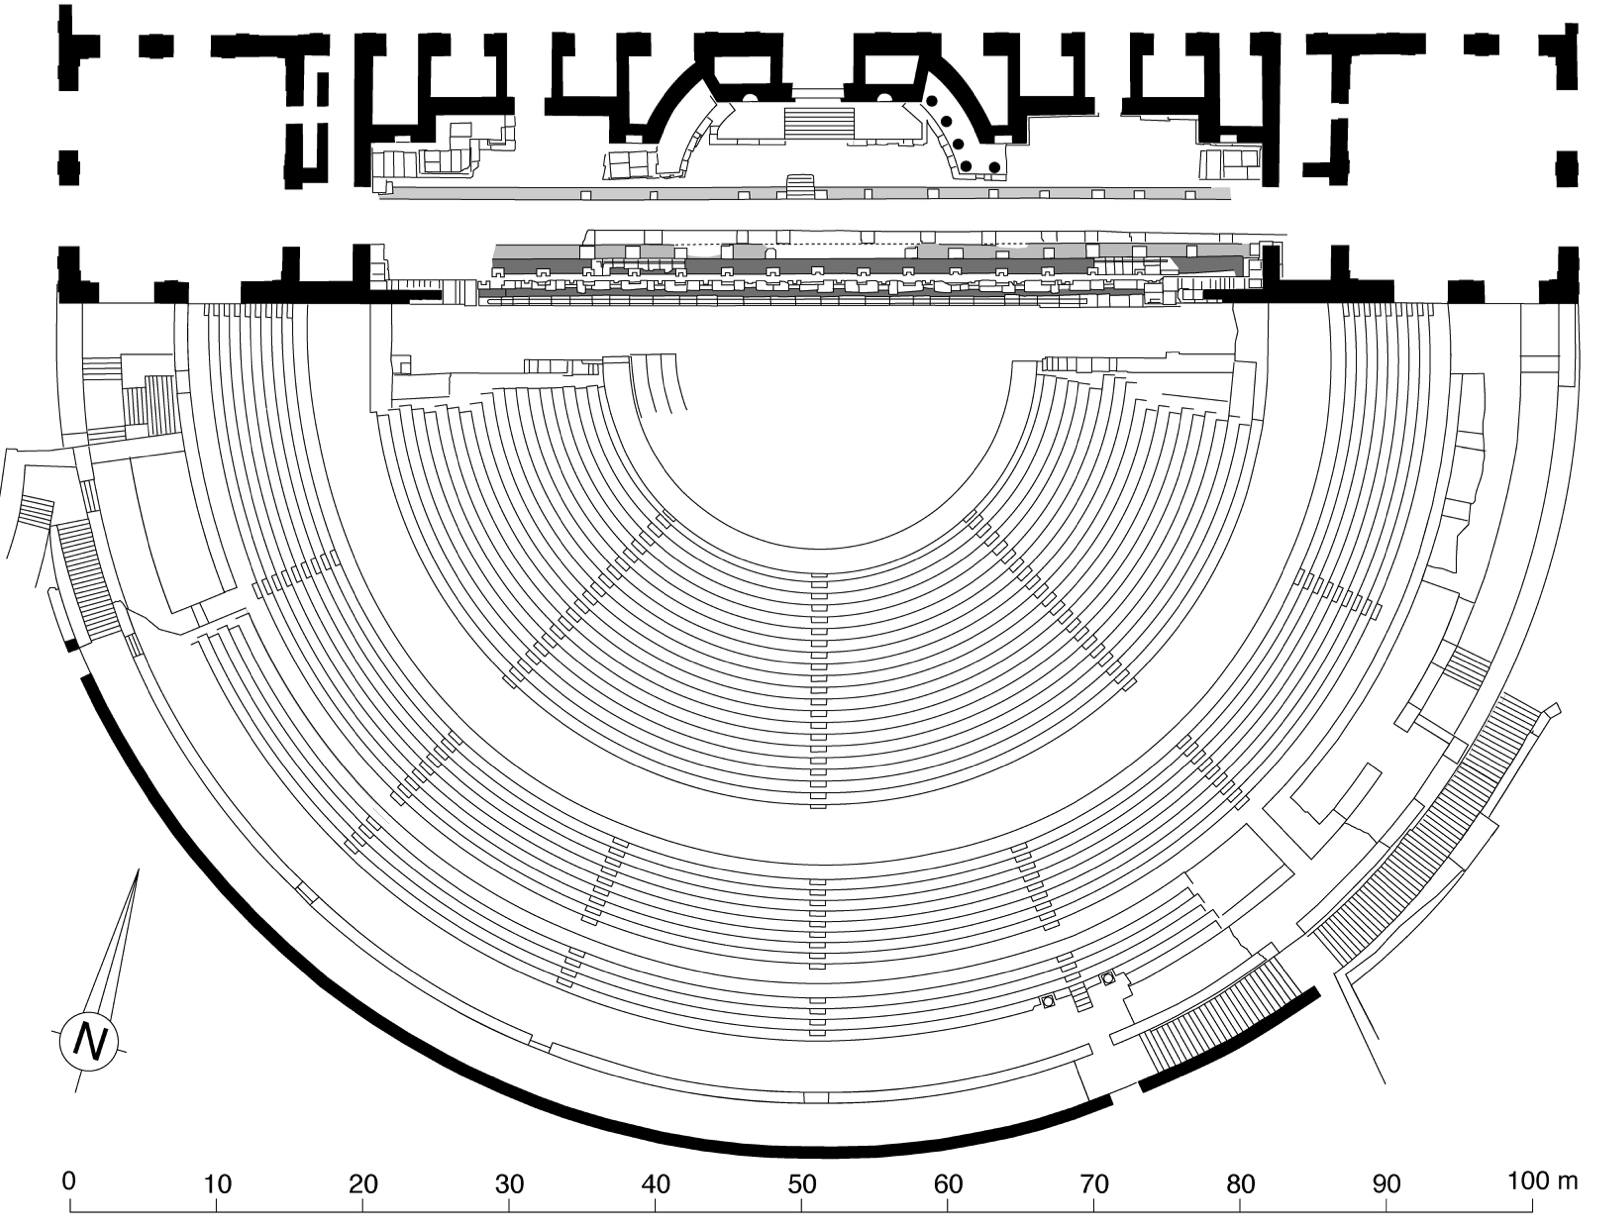
\includegraphics[width=\linewidth]{images/3emeniveau}
		\caption[Vue de dessus - 3ème niveau]{Plan du théâtre au niveau de la rue périphérique \footnotemark }
		\label{3emeniveau}
	\end{figureth}	
	\citefnt[Pl. XIX et XX fusionnées]{orangePl}
		
\section{Les couvertures et le \gls{velum}}
		
	\subsection{La couverture des \glspl{basilique} et du \gls{parascaenium}}
	\label{couverture-basi}
		
		La toiture qui couvre aujourd'hui les \glspl{basilique} et le \gls{parascaenium} (installée en 2006) reflète à peu près la proposition de restitution d'A.Caristie, à savoir un toit à double pente avec \gls{aretier} sur la diagonale partant de l'angle du mur arrière. L'étude de l'\gls{iraa} \cite[p. 36]{orangeTxt} tend à corriger cette hypothèse en supposant plutôt la présence de deux toitures successives et, au-dessus de la cage d’escalier, d’un petit toit à double-pente permettant non pas d’accéder aux combles mais au toit lui-même (fig. \ref{couvertureBadie}). Cette dernière hypothèse s'appuie sur des traces symétriques situées au-dessus de la cage d’escalier orientale et donne de nouvelles pistes aux archéologues sur la façon dont travaillaient les architectes de l'antiquité, et les moyens d'entretien du bâtiment dont ils disposaient. 
		
		\begin{figureth}
			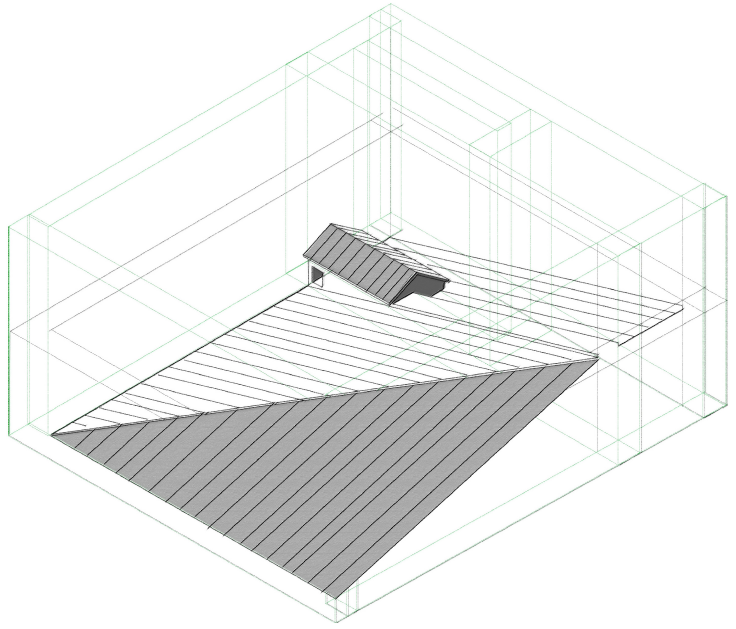
\includegraphics[width=0.7\linewidth]{images/couvertureBadie}
			\caption[Toitures de basiliques par A.Badie]{Proposition de restitution des toitures de la \gls{basilique} occidentale, de la cage d'escalier et du \gls{parascaenium} \footnotemark}
			\label{couvertureBadie}
		\end{figureth}	
		\citefnt[Pl. XLVII]{orangePl}
		
		\subsection{La couverture du \gls{postscaenium} et du \gls{pulpitum}} \label{couverture}
		
		Comme les toitures des \glspl{basilique} évoquées précédemment, le \gls{postscaenium} et le \gls{pulpitum} possèdent une couverture récente, cette fois réalisée en métal. Le choix de cette toiture reste sujet à controverse car bien que l'acier présente de nombreux avantages face au bois (poids, résistance au temps, etc), il dénature l'aspect du bâtiment en plus d'être anachronique. La version antique n'a laissé aucun vestige en elle-même car elle devait être faite en matériaux périssables et semble avoir subi un ou plusieurs incendies au cours de son histoire. Néanmoins les études de A.Caristie (fig. \ref{toitCaristie}) puis de l'\gls{iraa} (fig. \ref{toitBadie}) par la suite permettent d'entrevoir la forme de cette couverture. Premièrement, on distingue dans la partie sommitale du mur de scène des cavités d'encastrement permettant d'accueillir la charpente de la toiture, elles-même couronnées par une série de déversoirs par lesquels s’échappait l’eau de pluie. Deuxièmement, on peut observer une saignée sur le mur occidental indiquant la pente de la partie supérieure de la charpente (voir fig. \ref{toitBadie}). Troisièmement, on constate que le mur sud du \gls{postscaenium} (le front de scène) se terminait avec une pente de 19°, d'après les marques laissées par un incendie sur les murs latéraux. Celles-ci reflète la pente inférieure de la toiture. A.Carsitie a proposé une restitution de la couverture (fig. \ref{toitCaristie}) en s'inspirant des grues en bois utilisées à son époque et précise qu'il s'agit de \textit{"la combinaison qui"} lui \textit{"a paru la plus vraisemblable, sous le rapport de la construction, pour la couverture du proscenium sans prétendre cependant que ce soit la seule solution possible de cette intéressante question"} \cite[p. 31]{orangeTxt}. Effectivement, l'\gls{iraa} \cite[p. 32]{orangeTxt} conteste la forme triangulaire proposée par A.Caristie en faveur d'une forme parallélépipédique qui semble plus vraisemblable compte tenu du parallélisme des traces évoquées précédemment (fig. \ref{toitBadie}). Par ailleurs, cela coïncide avec la présence d'ouvertures au sommet des murs latéraux, permettant probablement d'atteindre la partie antérieur du comble, alors que la proposition d'A.Caristie les obstruait partiellement. Cette forme de toiture semble d'autant plus plausible au plan architectural qu'il en a été retrouvé des similaires dans les archives d'autres monuments \cite[fig. 27]{orangeTxt}. Cependant, il a été constaté que les cavités d'encastrement ont été plusieurs fois ajustées, agrandies ou rétrécies, ce qui suppose qu'il y aurait eu plusieurs toitures installées au cours de la "vie" du bâtiment. Notre étude pourra ainsi permettre d'en restituer différentes versions et de les comparer entre elles.
		
		\addtocounter{footnote}{1}
		\begin{figureth}
			\begin{subfigureth}{0.49\textwidth}
				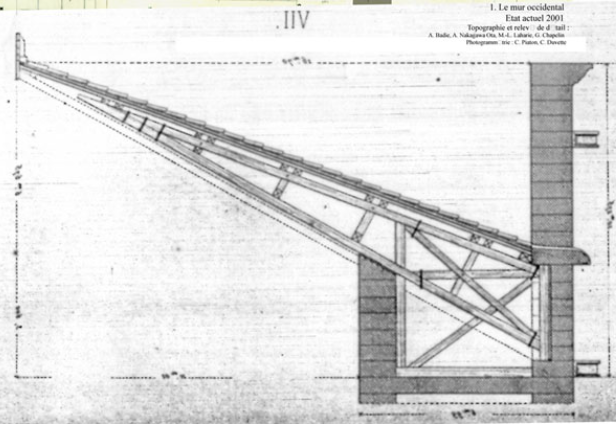
\includegraphics[width=\linewidth]{images/toitCaristie}
				\caption[Couverture de scène proposée par A.Caristie]{Proposition de restitution de la couverture de la scène par A.Caristie \footnotemark[\value{footnote}]}
				\label{toitCaristie}
			\end{subfigureth}	
			\begin{subfigureth}{0.49\textwidth}
				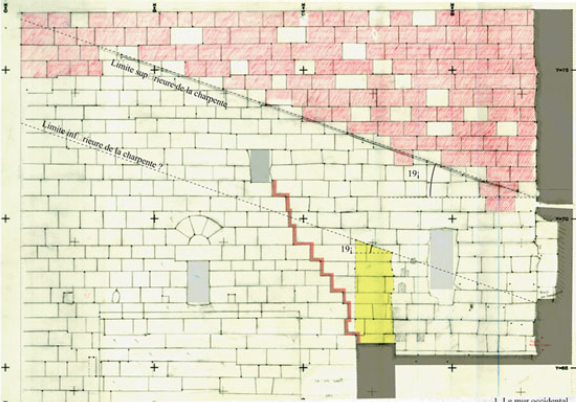
\includegraphics[width=\linewidth]{images/toitBadie}
				\caption[Relevé de la partie sommitale du retour ouest du front de scène]{Relevé de la partie sommitale du retour ouest du front de scène \footnotemark[\value{footnote}]}
				\label{toitBadie}
			\end{subfigureth}
		\end{figureth}
		\citefnt[fig. 24]{orangeTxt}
		
		\subsection{La couverture de la \gls{cavea}} \label{section velum}
		
		Il est reconnu que les théâtres romains possédaient généralement un appareillage permettant de déplier au dessus des spectateurs de longues toiles appelées \textit{vela} et communément assimilées à un ensemble unique : le \gls{velum}. Celui-ci permettait aux spectateurs d'être protégés du soleil et se déployait probablement partiellement en suivant le déplacement de l'astre notamment pour garantir une bonne ventilation. On peut lire dans la traduction de Vitruve\cite[p. 38]{vitruve} que "\textit{Comme il n'y avait que les portiques et le bâtiment de la scène qui fussent couverts, on était obligé de tendre, sur le reste du théâtre, des voiles soutenues par des mâts et des cordages, pour défendre les spectateurs de l'ardeur du soleil}". Nous savons par ailleurs d'après Pline l'ancien \cite[V-VI]{pline} que ce fut après Cléopâtre qu'on fit usage des toiles de lin pour donner de l'ombre dans les théâtres : "\textit{Q. Catulus, le premier, les appliqua à cet usage quand il fit la dédicace du Capitole}". Nous avons déjà évoqué précédemment (voir section \ref{sect_postscaenium}) les \glspl{console} permettant d'accueillir les mâts auxquels étaient accrochés les cordages. Il y en a douze au niveau du mur de scène et vraisemblablement tout autour du mur périphérique de la \gls{cavea} (dont il ne reste malheureusement aucune trace). Les modèles les plus courants représentent le \gls{velum} par un anneau situé au dessus de l'\gls{orchestra} auquel sont attachés les cordages qui permettent de le hisser par un système de poulies. Nous avons vu que les machinistes se plaçaient probablement au niveau de la \gls{porticus isc} pour, dans un premier temps hisser l'anneau, puis ensuite, déployer certaines \glspl{velum} au moment approprié.  
		
		Le théâtre d'Arles présente un certain nombre de trous au niveau de son premier gradin qui semblent avoir accueilli des mâts de soutien pour le \gls{velum} \cite[p. 38]{formige}. \`{A} coté de ceux-ci on trouve de plus petits trous probablement utilisés pour fixer les cordes. Cette particularité a peu été observée par ailleurs. Elle pourrait être due à la présence d'un fort mistral dans cette région et donc pourrait également avoir été mis en place à Orange. 

		
	\begin{figureth}
		\begin{subfigureth}{0.35\textwidth}
			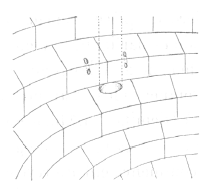
\includegraphics[width=\linewidth]{images/velumArles}
		\caption[Traces de mâts et de leur accroche dans les gradins du théâtre d'Arles]{Traces de mâts et de leur accroche dans les gradins du théâtre d'Arles \footnotemark}
			\label{velumArles}
		\end{subfigureth}	
		\qquad
		\begin{subfigureth}{0.55\textwidth}
			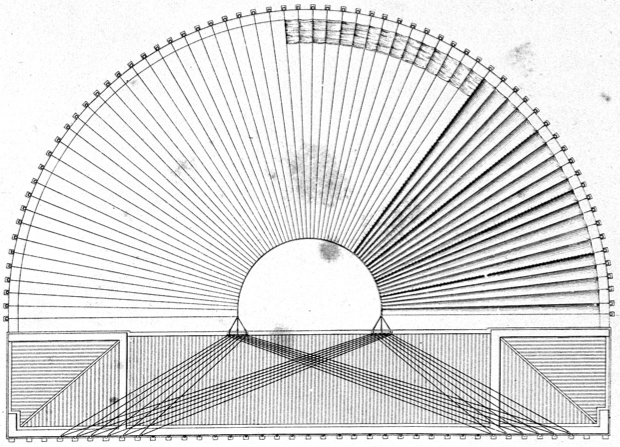
\includegraphics[width=\linewidth]{images/velumCaristie}
		\caption[Proposition de restitution du velum d'Orange par A.Caristie]{Proposition de restitution du velum d'Orange par A.Caristie \footnotemark}
		\label{velumCaristie}
		\end{subfigureth}
	\end{figureth}
\addtocounter{footnote}{-1}
\citefnt[fig. 5]{formige}
\addtocounter{footnote}{1}
\citefnt[Pl. VI]{orangePl}
				

		A.Caristie propose une restitution de \gls{velum} avec un anneau semi-circulaire et 67 mâts autour de la \gls{cavea} (fig. \ref{velumCaristie}). Nous verrons dans la section \ref{sect_velum} que ce chiffre ne coïncide pas avec ses autres dessins.
		














\chapter{Modélisation}
		\citationChap{
			Les détails font la perfection et la perfection n'est pas un détail
		}{Léonard de Vinci}
		\minitoc
		\newpage
		
		\section{Introduction}
		Pour pouvoir étudier un monument dans ces moindres détails, de nombreux chercheurs s'orientent aujourd'hui vers la modélisation 3D. Effectivement, jusqu'à ces quelques dernières années, les analyses architecturales antiques étaient principalement menées à l'aide de plans, de dessins, ou bien de maquettes à échelle réduite. Cependant, les outils numériques disponibles aujourd'hui comportent de nombreux avantages par rapport à ces anciennes techniques. Tout d'abord, il est possible d'obtenir les mêmes informations qu'avec des dessins ou des maquettes en terme de côtes, formes, aspect. Par ailleurs, la technologie numérique apporte au chercheur un nouveau champ d'observation et de nouveaux outils de travail. \textit{"En effet, il est clair que si les modèles 3D étaient à l’origine de simples outils d’aide à la visualisation et à la diffusion de contenu scientifique au grand public, le processus de modélisation tridimensionnelle doit maintenant être considéré comme une méthode qui offre la possibilité de faire de nouvelles découvertes."} \cite[p. 246]{rocheleau}.
		
		Premièrement, un modèle numérique permet d'archiver la quasi totalité des informations en un document unique. Le mode d'affichage que l'on choisira pourra être adapté à la cible de la présentation. \textit{"L’image n’est qu’un élément d’un discours qui doit, dans son ensemble, être pertinent vis-à-vis du public auquel il s’adresse."} \cite[p. 20]{golvin}. On peut donc par exemple observer un monument par vue du dessus avec ses cotes et en étudier ainsi le plan topographique 2D correspondant. De la même manière, il sera possible de réaliser une impression 3D de l'objet pour en avoir une maquette physique à l'échelle réduite. Ainsi, \textit{"la maquette électronique répond à l’une des critiques qui avaient été adressées aux maquettes rigides ; elle est capable de montrer les documents, les arguments, les hypothèses sur lesquels la restitution architecturale s’est fondée."} \cite[p. 26]{golvin} ce qui lui confère une force supplémentaire. Par ailleurs, la précision et la qualité des documents est largement renforcée par la manipulabilité des modèles numériques. La précision est alors celle des ordinateurs, soit, inférieure à $10^{-4}$ dans le pire des cas \cite[Tableau : Valeur pour les unités matérielles standard d'arithmétique à virgule flottante]{precisionmachine}. 
		 
		 Deuxièmement, un modèle numérique 3D peut être utilisé par des logiciels de calcul ou de simulation afin de tester des comportements physiques. On citera comme exemple les écoulements de fluide, l'ensoleillement ou la propagation d'ondes sonores. Il en est de même pour les questions architecturales d'agencement de décor ou de portance par exemple. Ce type d'outil permet également de réaliser des animations (déplacement de personnages, ouverture de haut-vents, ...) ou des visites immersives grâce aux technologies de réalité virtuelle. On peut alors visualiser l'objet d'étude dans son ensemble ou bien partie par partie à l'aide de technologies telles que les écrans 3D, les caves (écrans géants parabolique ou cubiques) ou les casques de réalité virtuelle. Cela apporte un point de vu immersif quasi inatteignable sans la technologie numérique.
		 
Il existe bien entendu de nombreuses limites à la numérisation 3D car cette technique est relativement récente (quelques dizaines d'années) et beaucoup de développements sont en cours. La principale contrainte est la puissance de calcul des ordinateurs et leurs espaces de stockage qui doivent prendre en charge de très grandes quantités de données.

Pour virtualiser des monuments, nous citerons deux techniques parmi les plus souvent utilisées. La première consiste à réaliser un nuage de point à l'aide d'appareils de mesure (laser, appareils photo, ...) à la manière d'un scanner. Prenons l'exemple de la photogrammetrie qui est aujourd'hui largement répandue dans la restitution numérique de monument. Il s'agit de photographier l'ensemble du bâtiment sous tous ses angles, en s'assurant que chaque photo a une partie commune avec une autre. Les logiciels de traitement peuvent alors corréler les photos les unes avec les autres et recréer l'image en trois dimensions. Cependant, la limite de cette technique est que, plus la précision est grande, plus le volume de données à traiter est conséquent, ce qui rend les calculs plus difficiles. C'est pour cette raison que nous avons utilisé la deuxième méthode dite de \gls{cao}. Il s'agit de retranscrire l'architecture du monument par des formes géométriques 3D plus ou moins complexes.

Dans ce chapitre nous allons présenter comment le théâtre antique d'Orange a été modélisé, quelles ont été les difficultés soulevés et les astuces utilisées. Il sera précisé quelles sont les informations architecturales et archéologiques que concaténe le modèle numérique, ainsi que les sources qui ont permis de les implémenter.
Avant de détailler uns par uns les éléments modélisés, nous ferons un point sur la méthodologie entreprise durant le projet.


\section{Méthodologie}

Il existe de nombreux projets ayant pour objectif de virtualiser des monuments antiques. On citera par exemple le projet de virtualisation basé sur "le plan de Rome" de Paul Bigot. Il s'agit d'une maquette de plâtre de $70m^2$, à l'échelle 1/400, représentant une partie de la Rome de Constantin (IV\up{e} siècle après JC). Ce projet est mené par le \gls{cireve} depuis plus de dix ans et a pour but d'utiliser la réalité virtuelle comme outil de recherche archéologique \cite[p. 157-158]{fleury}. Ce type d'étude commence toujours par un état des lieux bibliographique et le choix de la temporalité. Comme nous l'avons vu dans la section \ref{introarcheo}, un monument de cette ancienneté subit de nombreuses transformations au cours de sa vie. Il est donc primordial de situer dans le temps la représentation qui sera faite du bâtiment. Nous choisissons pour notre part de restituer le théâtre d'Orange dans son état au premier siècle de notre ère, c'est à dire dans ses toutes premières années de vie. Néanmoins nous ne pouvons nous baser que sur les relevés actuels ayant subit les effets du temps et les manipulations humaines, le résultat ne pourra donc être qu'approché.


La deuxième étape de ce travail de modélisation est de choisir l'outil qui permettra de la réaliser. Comme indiqué en introduction de ce chapitre, nous utilisons la technique de \gls{cao} car nous avons besoin d'un maillage "léger" (notamment pour les simulations acoustiques de la deuxième partie du projet). Avec un monument comme le théâtre d'Orange, on atteint déjà des dizaines de milliers d'éléments. Cela reste malgré tout bien moindre qu'avec un nuage de points qui aurait constitué des millions d'éléments. Par ailleurs, notre étude porte dans un premier temps sur les formes géométriques du théâtre. Il sera possible d'y greffer, dans un deuxième temps, des éléments plus précis réalisés par photogrammetrie. Ce fut d'ailleurs l'un des buts premier à l'initiative de ce projet de thèse. Il a notamment été numérisé en 2015, par photogrammétrie, une partie des fragments de la frise dionysiaque retrouvés dans les décombres. La dernière raison qui nous pousse à modéliser le monument par \gls{cao} est que la "photogrammétrisation" du lieu aurait apporté beaucoup d'informations erronées pour la restitution du bâtiment dans son état d'origine. Effectivement, les restaurations ayant été conséquentes notamment sur la partie  \gls{cavea} et l'érosion ayant quelque peu dégradé les façades, la restitution aurait de toute façon dû subir une large étude documentaire pour compléter le modèle. Par ailleurs une campagne de mesure par photogrammètrie ou lasergrammetrie est très longue et fastidieuse, ce qui aurait retardé d'autant plus le projet. La technologie de \gls{cao} est largement répandue depuis une trentaine d'années et le nombre de logiciels permettant d'utiliser cette méthode est conséquent. Voici quelques exemples parmi les plus connus : \textit{AutoCAD, CATIA, SketchUp, 3DSMax}. Après une étude comparative, le choix s'est porté sur le logiciel \textit{Blender} car celui-ci possède l'avantage d'être :

\begin{itemize}
	\item gratuit
	\item multiplatforme (Windows, Mac, Linux)
	\item modulaire (de nombreuses fonctionnalités peuvent y être ajoutées selon les besoins)
	\item suivi et commenté par une large communauté
\end{itemize}

Par ailleurs, Blender : 
\begin{itemize}
	\item permet un rendu réaliste (voire photo-réaliste) notamment grâce au texturage
	\item permet de réaliser des animations et des vidéos
	\item utilise des effets physiques tels que : la gravité, la déformation de type tissu, l'écoulement de fluides ...
	\item peut exporter les maillages sous différents formats couramment utilisés (obj, fbx, stl, ...)
	\item permet le développement de scripts en python
\end{itemize}

Toutes ces spécificités vont être utilisées dans le projet et c'est pourquoi c'est ce logiciel qui a été choisi. Il comporte néanmoins quelques limites, notamment sa difficulté de prise en main, le fait qu'il soit peu utilisé dans le milieu architectural et que son "\textit{game engine}" soit de moins bonne qualité que certains de ses concurrents (Unity ou Unreal Engine par exemple). Le "\textit{game engine}" est le moteur de jeu vidéo permettant de se déplacer dans l'environnent avec un personnage ou bien en vue subjective. Néanmoins, ce point n'est pas bloquant car Blender peut exporter des modèles texturés dans Unity ou Unreal pour des visites virtuelles de très haute qualité. Par ailleurs Blender, comme tous les logiciels de CAO, propose toute une gamme d'outils mathématiques permettant de modifier les objets. Voici quatre exemples qui vont être beaucoup utilisés lors de la modélisation du théâtre d'Orange :

\begin{figureth}
	\begin{subfigureth}{0.45\textwidth}
		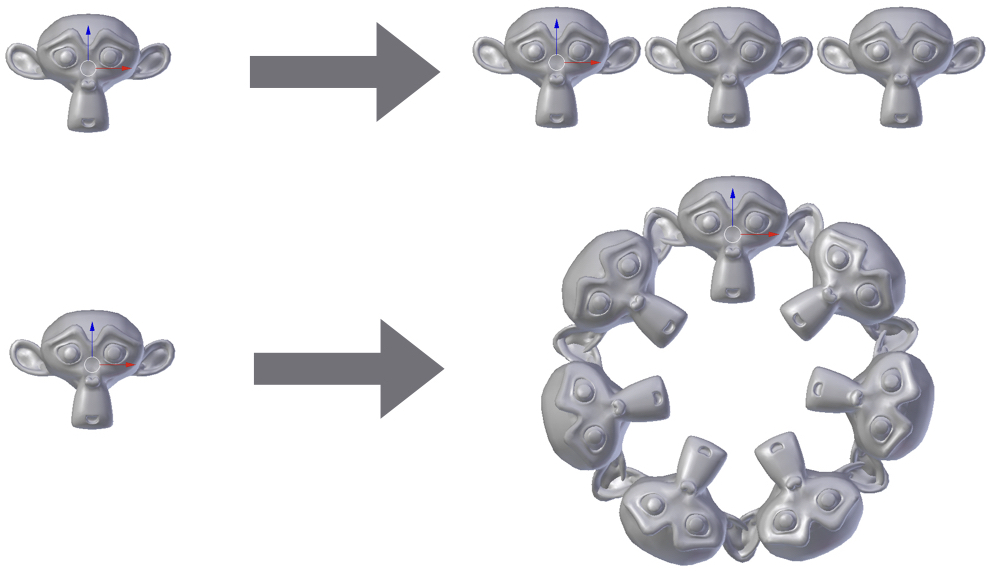
\includegraphics[width=\linewidth]{images/array}
		\caption{\gls{array}}
		\hfill
		\qquad
	\end{subfigureth}
	\qquad
	\begin{subfigureth}{0.45\textwidth}
		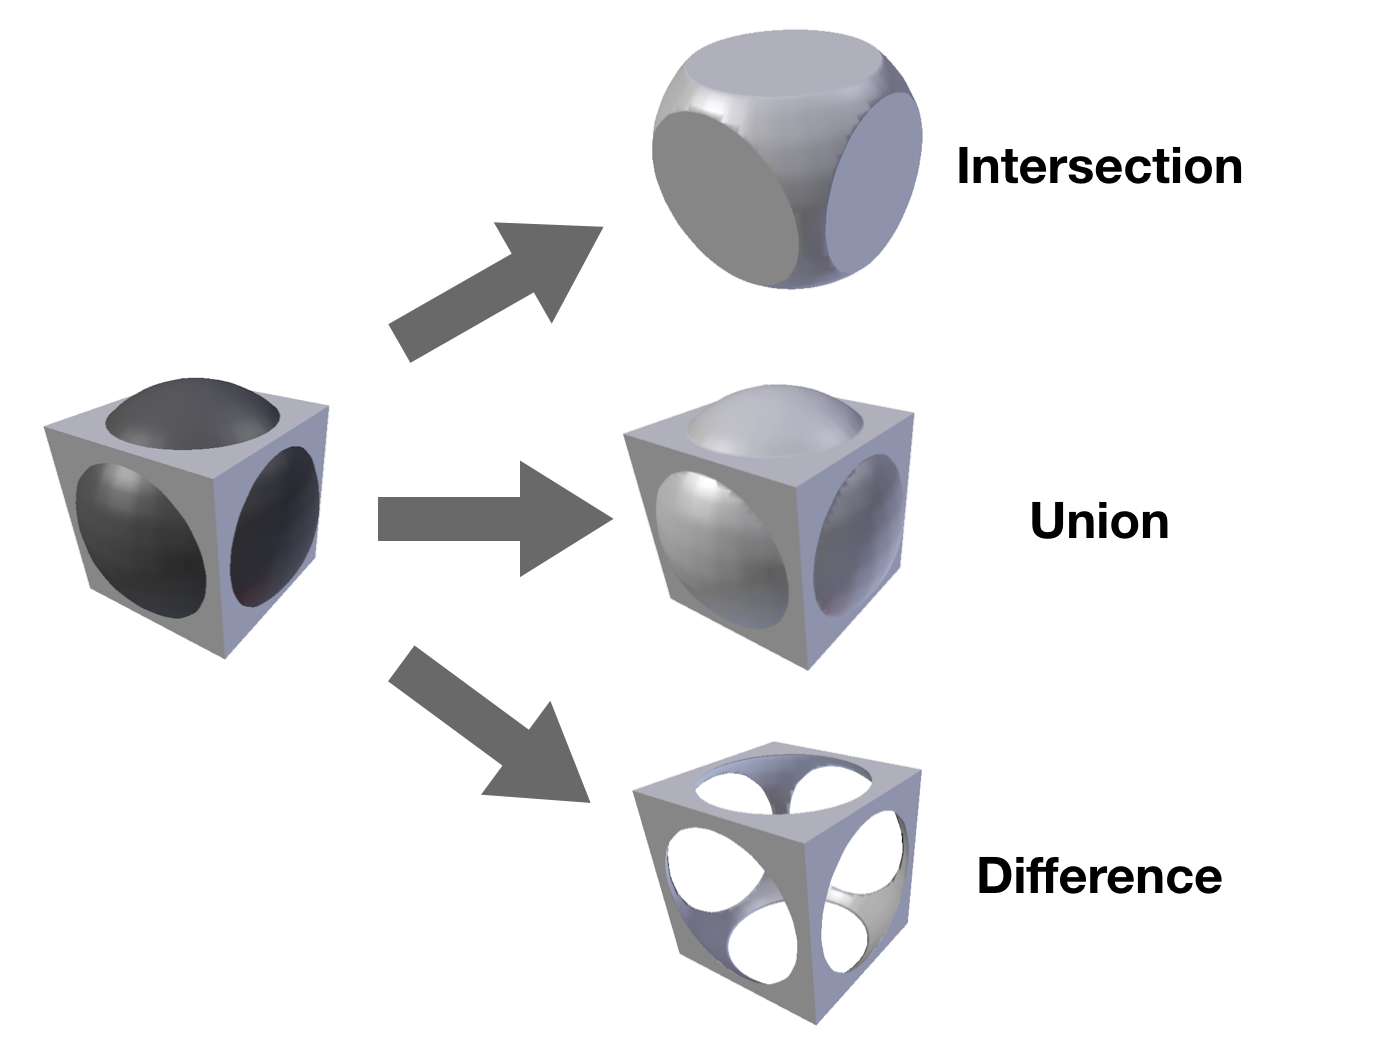
\includegraphics[width=\linewidth]{images/boolean}
		\caption{\gls{boolean}}
		\qquad
	\end{subfigureth} 
	\begin{subfigureth}{0.45\textwidth}
		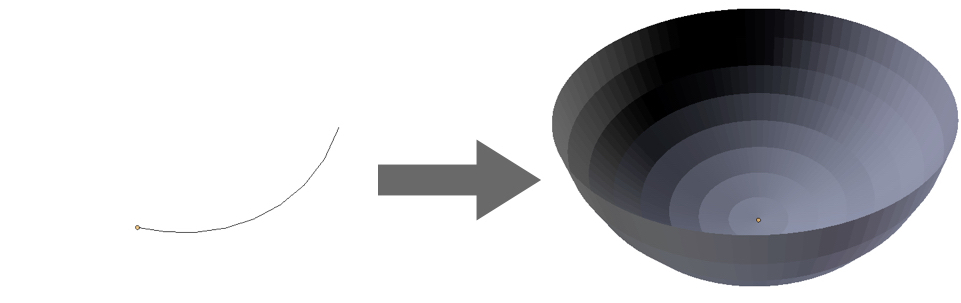
\includegraphics[width=\linewidth]{images/screw}
		\caption{\gls{screw}}
	\end{subfigureth}
	\qquad
	\begin{subfigureth}{0.45\textwidth}
		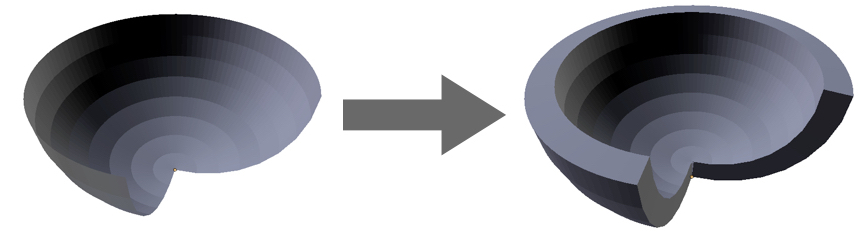
\includegraphics[width=\linewidth]{images/solidify}
		\caption{\gls{solidify}}
	\end{subfigureth}
\caption{Illustration de quatre exemples de \gls{modifier} Blender}	
\end{figureth}		

L'intérêt d'utiliser de tels outils est de pouvoir effectuer sur les objets des modification non permanente. Nous verrons par exemple que les gradins ne sont qu'un simple plan de forme quasi-triangle auquel on affecte tout un panel de \glspl{modifier}.\\

Pour modéliser le théâtre, il faut d'abord le voir dans son ensemble pour pouvoir le situer dans son repère. Globalement, et comme tous les théâtres romains, le théâtre d'Orange a une enveloppe extérieure en forme de U fermée par un mur rectiligne. Sa \gls{cavea} est construite sur le flan d'une colline, qui sera pour sa part, créée dans un deuxième temps (contrairement à la construction réelle du théâtre). 

On choisi de prendre l'axe X pour la direction sud-nord et l'axe Y pour la direction ouest-est. Sur le plan XY, c'est à dire le plan de l'horizon on choisi le point (0,0) au centre du demi-cercle formé par la \gls{cavea}. Nous faisons ce choix car cette dernière possède un centre de révolution, et il sera plus pratique par la suite, notamment au moment d'appliquer des outils automatiques, de placer celui-ci au centre du repère de Blender. Concernant l'axe Z portant les informations d'élévation, nous utiliserons les relevés d'altitude, présents dans le rapport de l'\gls{iraa} \cite[Pl. XXIX, XLIV, XLVIII, XLIX, LX]{orangePl}, et donnant des élévations géoréférencées par rapport au niveau de la mer. Le plan supérieur de l'\gls{orchestra}, par exemple, se trouve donc à 40m sur l'axe des Z. Le modèle est réalisé à l'échelle 1, ce qui signifie que les cotes apparaissant sur Blender sont les cotes réelles. Par ailleurs, certaines d'entre elles proviennent de relevés effectués sur le terrain, et sont donc fidèles à l'architecture du bâtiment au cm près. D'autres, seront des valeurs moyennes, approchées, ou bien calculées, et cela sera bien entendu précisé. \textit{"Le chercheur confronté au problème de la restitution d’un site est obligé de considérer trois types de données : les données connues, les données cachées, les données détruites."} \cite[p. 27]{golvin}. Effectivement, le but de ce projet étant de restituer le théâtre dans sa version d'origine, il faudra discriminer les données antiques de celles produites par la restauration de Formigé. Nous travaillerons ainsi sur des éléments complètement disparus, comme la \gls{porticus isc} ou le \gls{velum}, uniquement à partir d'hypothèses de restitutions. Les différents éléments présentés dans ce document apparaissent dans l'ordre logique de leur modélisation.

Il est important de noter que la modélisation a été faite par rapport à des plans qui peuvent être affichés en transparence sur Blender pour les superposer au modèle. On dispose alors du résultat ainsi que des sources dans un seul et même fichier.

\section{La  \gls{cavea} et ses substructures}  
	\label{La cavea et ses substructures}

\begin{figure}[!h]
	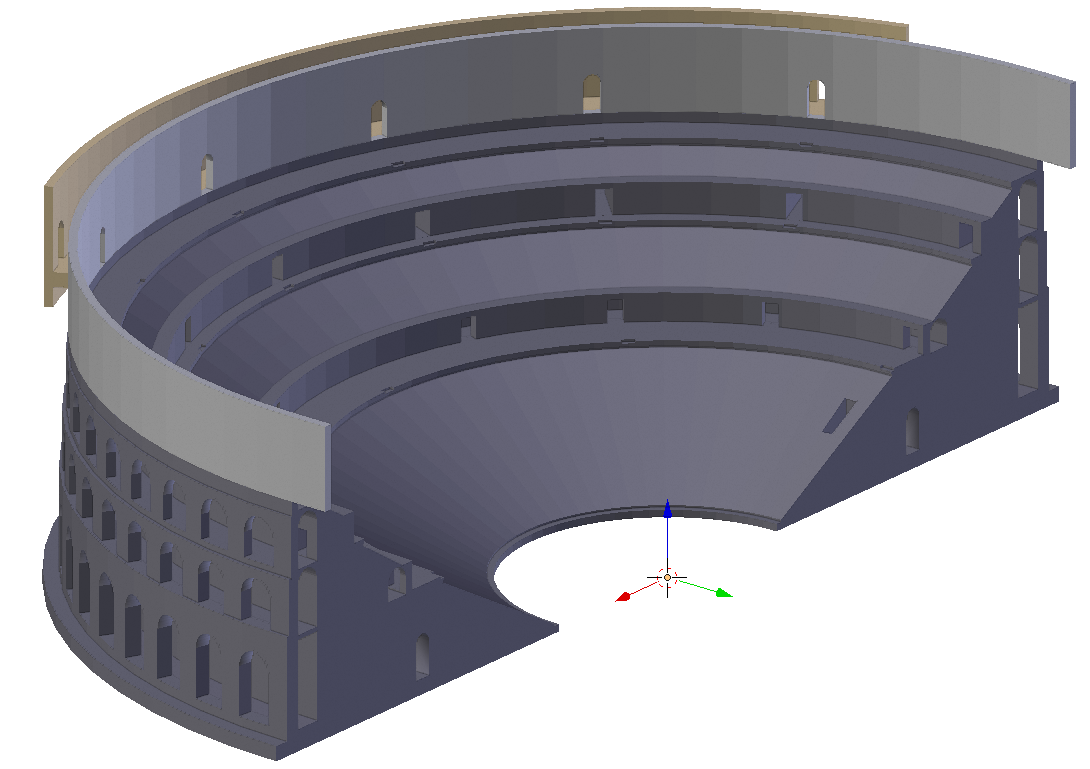
\includegraphics[width=\linewidth]{images/modCavea}
	\caption{Modélisation de la \gls{cavea}} 
	\label{modCavea} 
\end{figure} 

La \gls{cavea} est le premier élément que nous modélisons car, comme stipulé précédemment, son centre de révolution est situé à l'origine du repère XY. La modélisation se fait à partir de la figure \ref{coupeCavea}. La première chose à noter est que sur ce plan, on ne connait pas la distance par rapport au centre de révolution. Par contre, on sait que la paroi extérieure est au même niveau que la bordure des \glspl{basilique}, c'est à dire à 51,96m du centre (d'après la figure \ref{cotes}). Cette valeur est obtenue en prenant la moitié de la longueur totale du mur de scène. On part donc de cette paroi extérieure pour dessiner sur Blender la coupe de la \gls{cavea} en suivant les cotes indiquées. Cependant, plusieurs points posent difficulté. Premièrement les gradins sont représentés par des traits discontinus et sont donc hypothétiques. Leurs modélisations sont décrites dans la partie \ref{sect-maenianum}. Nous avons par contre besoin de connaitre précisément l'espace qui leur est dédié, afin de concevoir l'objet  \gls{cavea} qui leur sert de support. Nous obtenons ces valeurs en utilisant les quatre lignes de cotes horizontales. Or pour les deux lignes arrivant au niveau du mur du  \gls{podium} au dessus du deuxième \gls{maenianum}, on a deux informations contradictoires. D'une part, nous avons :
\begin{center}
$1,25+2,60+1,13+2,90+1,03=8,91m$
\end{center}
et d'autre part :
\begin{center}
$0,35+0,92+2,59+4,83=8,69m$
\end{center}
soit 22cm de différence. \\

Or on estime qu'il n'est pas crédible que le mur soit incliné de la sorte. Trois causes d'erreur sont possibles :
\begin{itemize}
	\item La mesure qui a été faite a été mal reportée et le document présente une coquille.
	\item Les mesures ne sont pas toutes effectuées sur un même plan de coupe, et d'un endroit à l'autre de la  \gls{cavea}, l'épaisseur des murs peut effectivement varier.
	\item La mesure est exacte mais les pierres s'étant érodées par endroit, on observe des fluctuations d'épaisseur qui n'étaient pas présentes à l'origine.
\end{itemize}

Pour trancher sur la décision nous adoptons la règle suivante :

\begin{theo}\label{epaisseur}
	Lorsque deux cotes sont contradictoires, on utilise celle correspondant à la plus grande épaisseur de pierre.
\end{theo}

Cela permet de trancher dans le choix des cotes tout en prenant en compte la possibilité que les pierres se soient érodées. Nous prenons dans un premier temps le parti pris de modéliser la  \gls{cavea} avec des cotes identiques sur tout son pourtour. 

Pour cette même longueur, A.Carisite (voir fig. \ref{caristieDessus}) donne des mesures encore différentes : 
\begin{center}
$4,55+2,70+0,95=8,20m$.
\end{center}
En ajoutant le décrochage de 35cm on obtient 8m55. \\

On voit donc bien que la \gls{cavea} ne pourra pas être modélisée avec une précision supérieure à quelques dizaines de centimètres en utilisant des cotes communes sur toute la circonférence. Pour obtenir un résultat plus réaliste, il faudrait effectuer de nouvelles campagnes de mesure en un nombre significatif de points. Néanmoins, les restaurations de la \gls{cavea} ayant été très conséquentes, il semble extrêmement difficile de remonter à la structure initiale avec grande précision.

Pour créer la substructure du troisième \gls{maenianum} nous appliquons donc la règle \ref{epaisseur} explicitée plus haut, et nous nous référerons au plan théorique \ref{coupeCavea} pour connaitre les élévations. Lorsque celles-ci ne sont pas chiffrées et qu'on ne les retrouve pas dans un autre document, nous obtenons la valeur par mise à l'échelle du plan. Nous modélisons également les trois niveaux de galeries qui seront solidaires à cet objet. Les caissons de soutènement situés sous le troisième \gls{maenianum} sont par contre modélisés séparément. Effectivement, contrairement à la \gls{cavea}, on ne va pas les extruder en un seul bloc sur 180° mais chaque caisson va être séparé de son voisin pour laisser l'espace des vomitoires. A.Caristie restitue dans ses plans six de ces caissons de soutènement (dont un incomplet) validant leur origine antique. Ainsi on utilise, à partir de la figure \ref{coupeCavea}, les cotes en deux dimensions de ces caissons que l'on répète huit fois avec un angle de 21,95°, et que l'on extrude à l'aide d'un \gls{screw} sur 19,2°. On fait ensuite subir une rotation globale à l'ensemble des huit caissons afin qu'ils soient symétriques par rapport à l'escalier central de la \gls{cavea} (quatre de chaque coté). 

Pour réaliser la substructure du deuxième \gls{maenianum} on complète le modèle afin que la première \gls{precinction} arrive à l'affleurement du mur de scène. Là encore on trouve un problème de cotes puisque, d'après la figure \ref{cotes}, la largeur de la basilique est de :
\begin{center}
$1,34+14,22+1,17+3,55+1,19=21,47m$.
\end{center}
Or on a : 
\begin{center}
$4,35+0,91+2,41+0,88+4,48=13,03m$.
\end{center}
En les ajoutant aux 8m91 déjà modélisés, on arrive à :
\begin{center}
$13,03+8,91=21,94m$
\end{center}
soit 47cm de différence. 


A.Caristie (fig. \ref{caristieDessus}) donne 8m entre les  \glspl{podium} du deuxième et du troisième niveau contre 8m68 pour M. Fincker et J.M Labarthe (fig. \ref{coupeCavea}). Les deux plans sont par contre cohérent à 5cm près concernant la largeur de l' \gls{ambulacre} ainsi que l'épaisseur de ses murs. C'est donc au niveau du remblai soutenant la partie supérieure du deuxième \gls{maenianum} que se trouvent les écarts de mesure. On part donc de l'angle de la basilique pour créer au premier niveau : la \gls{precinction}, le \gls{podium}, l'\gls{ambulacre} et son mur interne. Au deuxième niveau, la \gls{precinction} du deuxième niveau est par contre créée à partir du  \gls{podium} car on connait sa longueur et son élévation. Cela nous donne 7m96 entre les \glspl{podium} du deuxième et du troisième niveau, ce qui corrobore la valeur de A.Caristie.

Il reste la substructure du premier \gls{maenianum}. Ici encore la longueur des gradins n'est pas stipulée. Par contre, A.Caristie (fig. \ref{caristieDessus}) nous dit que le repose-pied se trouve à 14m95 du centre de la \gls{cavea} et que le \gls{podium} du premier niveau se trouve 20m plus loin. On constate qu'en enlevant les 4m35 de la première \gls{precinction} aux 34m94 de A.Caristie, on obtient 30m59. Cette valeur est proche de la demie-longueur du mur de scène auquel on ôte la basilique : 
\begin{center}
$51,96 - 21,47=30,49m$.
\end{center}

Il ne manque que l'information de la largeur du marche-pied et de la couverture du caniveau pour connaitre l'espace réservé au premier \gls{maenianum} et terminer cette partie. Ces dimensions sont obtenues par mise à l'échelle des plans \ref{coupeCavea} et \ref{caristieDessus}. Il reste également un doute sur le fait que la \gls{precinction} arrive bien à l'affleurement de la basilique, puisque ce n'est pas le cas sur la représentation de la coupe des \glspl{aditus} (voir fig. \ref{aditusOccidental} et \ref{aditusOriental}).

Une fois ce plan de coupe réalisé on utilise le \gls{screw} sur 90° et le \gls{mirror} pour obtenir un objet en volume sur un hémicycle. Le \gls{mirror} permet de s'affranchir d'une étape au moment de fermer le maillage. Effectivement, pour pouvoir créer les arcades, les vomitoires et autres ouvertures, il faudra avoir un maillage fermé. Or, la présence des différentes galeries empêchent de créer simplement une face pour fermer la structure, il faut en créer plusieurs. En effet, Blender ne comprend pas quels points sont à relier ensemble si le problème n'est pas subdivisé. Il faudra donc créer des faces dont les bords sont concaves. L'utilisation du \gls{mirror} permet de n'effectuer cette opération que sur un seul des cotés de l'objet. Appliquer le \gls{screw} et fermer le maillage sera indispensable par la suite pour utiliser le \gls{boolean}.

Cette structure va donc pouvoir être percée par différents objets, à commencer par les arcades donnant sur l'extérieur. Celles-ci sont créées en élévation grâce au plan de coupe théorique (fig. \ref{coupeCavea}). Leur largeur de 3,419m est donnée par le plan de A.Caristie (fig. \ref{caristieDessus}). On estime que l'entrée des \glspl{aditus} est également de cette largeur et s'élargit par la suite au niveau des \gls{parodos}. On peut considérer que les arcades des trois niveaux ont une hauteur différente mais une largeur identique, notamment car les parois internes des \glspl{aditus} ne présentent pas de marque contredisant cette hypothèse. Si les arcades avaient fait tout le tour de la  \gls{cavea}, c'est à dire dans le cas où il le théâtre n'aurait pas été adossé à une colline, il y aurait eu 31 arcades sur chaque niveau. C'est le résultat que l'on obtient en prenant l'hypothèse que la largeur des arcades est constant tout comme leur espacement. Cela corrige le plan de A.Caristie qui lui, présente 33 arcades sur toute la périphérie. Un triplet d'arcades verticales, placé au niveau de l'\gls{aditus} oriental, est alors répété à l'aide d'un \gls{array} de manière circulaire autour du centre de la \gls{cavea} avec un angle de 6,13°. Leur nombre est paramétrable et importe peu puisque la colline viendra en masquer une partie, par contre, les arcades orientales devront être reflétées en miroir sur la partie occidentale. Effectivement, l'arcade de références étant sur la partie rectiligne de la \gls{cavea}, on ne peut pas utiliser la rotation sur 180° car la dernière n'arriverait pas dans l'axe. On peut fixer à 15 le nombre de triplet d'arcades de chaque coté de la \gls{cavea} dans un premier temps (c'est à dire toutes sauf celle dans l'axe) et lorsqu'on appliquera les \glspl{modifier}, on supprimera celles qui sont complètement occultées par la colline. Ne pas mettre l'arcade centrale permet de visualiser l'effet de la soustraction sur la \gls{cavea} avant l'application des \glspl{modifier}. Effectivement, avec une seizième arcade on aurait une superposition de deux objets identiques au niveau du miroir et cela est mal géré par Blender dans un \gls{boolean}. 

 Au niveau de la première et deuxième \gls{precinction}, on perce la structure à l'aide d'un nouveau \gls{boolean} pour créer les \glspl{vomitorium} qui permettent d'accéder aux  \glspl{ambulacre}. La forme qui va être soustraite à la \gls{cavea} se compose d'un pavé droit créant un trou rectangulaire au niveau du \gls{podium}, puis d'un demi-cylindre extrudé permettant de créer un couloir vouté allant jusqu'à l'\gls{ambulacre}. Le niveau bas est au niveau de la \gls{precinction}, et le niveau haut arrive à 50cm en dessous du  \gls{podium}, en considérant que l'espace au dessus du vomitoire est du même ordre de grandeur qu'un gradin. Ces passages sont disposés dans l'espace entre deux caissons. La forme de référence est donc répétée avec un angle de 21,95° grâce au \gls{array} et l'ensemble est pivoté de 2° autour de l'axe Z. 

Une porte venant des  \gls{aditus} permet aux spectateurs de se rendre à mi hauteur de l' \gls{ima cavea}. La modélisation de cette cage d'escalier est décrite dans la section \ref{sect-escaliers}, néanmoins, on note que l'"objet cavea" va être percée d'une ouverture permettant aux spectateurs de se rendre au dixième gradin.

Deux nouveaux objets séparés sont créés afin de modéliser la rue périphérique et ses murs intérieur et extérieur. Ils sont séparés de "l'objet cavea" afin de conserver une représentation fidèle au plan \ref{coupeCavea}. Le mur intérieur est simplement le duplicata d'une arrête de la paroi supérieure du mur extérieur de la \gls{cavea}, à laquelle on affecte les \glspl{modifier} "Screw" et "Solidify". Ceux-ci permettent de créer un mur circulaire sur la périphérie de la \gls{cavea} et de paramétrer sa hauteur. Aucune donnée ne nous permettant de connaitre l'élévation exacte de ce mur, nous laissons cette valeur modifiable dans le \gls{solidify}. Sur ce mur sont découpées quatre portes alignées avec les escaliers E9 à E12 (voir fig. \ref{2emeniveau}) conformément à la restauration de J-C.Formigé. Celles-ci auraient permis d'accéder à la \gls{porticus isc} depuis la rue périphérique et ne sont que de simple hypothèses. Elles sont d'ailleurs facilement modifiables grâce au \gls{boolean} qui rend la transformation non permanente. Grâce à un nouveau \gls{solidify} et un \gls{mirror}, ce mur est prolongé au dessus des \glspl{aditus}. La rue périphérique, ainsi que son mur extérieur, forment un objet séparé délimité par l'arrivée de deux escaliers périphériques représentés sur la figure \ref{3emeniveau}. Cet objet est pivoté de 21° autour de l'axe Z et s'étend sur 94° à l'aide d'un \gls{screw}. Ce dernier est appliqué définitivement afin de pouvoir retirer deux portes arquées alignées avec E9 et E12. Leur position est donnée sur la figure \ref{3emeniveau} et semble crédible d'après les restitutions de H.Daumet \cite[Pl. VII]{orangePl}. Leur forme est sous-entendue par la restitution de A.Caristie \cite[Pl. VI]{orangePl} mais reste hypothétique. Le mur extérieur se prolonge d'ailleurs sous le niveau du sol sur une longueur que l'on estime grâce à cette même référence. 


\section{Les  \glspl{maenianum}} \label{sect-maenianum}

\begin{figure}[!h]
	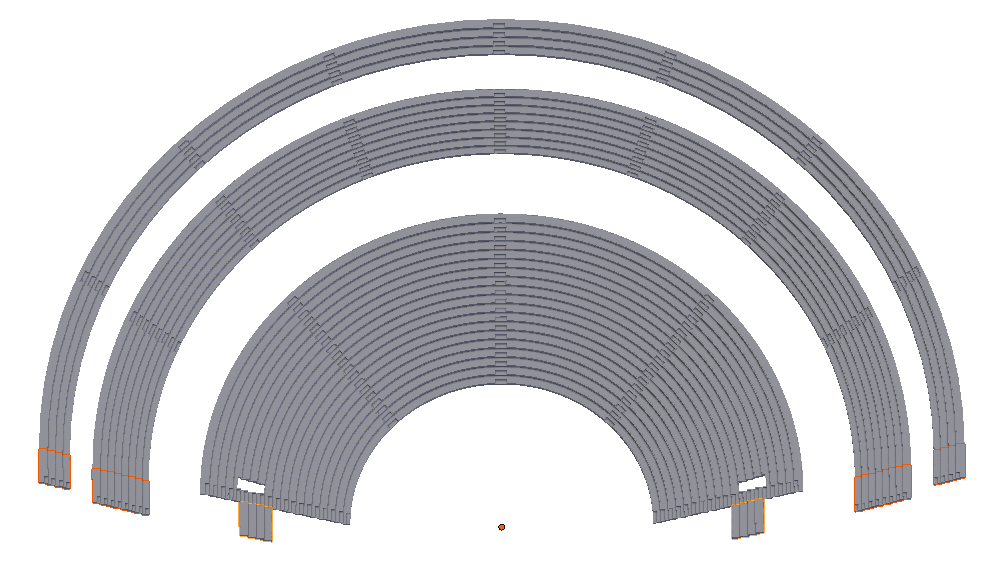
\includegraphics[width=\linewidth]{images/modMaenianum}
	\caption{Modélisation des \gls{maenianum}} 
	\label{modMaenianum} 
\end{figure} 

Les \glspl{maenianum}, c'est à dire les gradins, sont modélisés séparément de la \gls{cavea}. Chacun des trois \glspl{maenianum} est modélisé à partir d'un objet plan, de forme quasi-triangle, créé d'après la forme du morceau de gradin antique apparaissant dans le théâtre (voir fig. \ref{coupeGradin}). Les gradins étaient à priori assemblés à partir de blocs rectangulaires sciés en deux sur une diagonale décalée d'une dizaine de centimètres à partir de l'angle. Ce méplat permettait de poser les blocs les uns sur les autres. Le reste de leur longueur reposait sur de l'\textit{opus caementicium}, sorte de remblai constitué de mortier et de tout-venant qui n'est pas modélisé. 

On commence par créer le repose-pied dont on place l'extrémité à 14m95 du centre (fig. \ref{caristieDessus}). Sa largeur sera de 50cm dont 40cm apparents et 10cm recouverts par le premier gradin. Le premier gradin est donc placé à 15m35 du centre et possède un méplat de 10cm positionné au dessus du marche pied. La hauteur du gradin est des 45cm et sa partie haute mesure 89,6cm au total, dont 10cm recouvert par le gradin suivant. Celui-ci sera répété 19 fois avec un \gls{array} dont le décalage relatif est de 1 sur Z et 0,889 sur X (ce qui permet de positionner sur son méplat le gradin suivant). Le dix-neuvième gradin arrive ainsi à 30m59 du centre, ce qui permet bien à la \gls{precinction} de le recouvrir de 10cm comme s'il s'agissait d'un ultime gradin. De la même manière, pour le deuxième \gls{maenianum}, on place le premier gradin à 95cm du bord du \gls{podium} comme indiqué sur la figure \ref{coupeCavea} et on donne comme longueur 69cm apparents et 10cm recouverts par le prochain gradin. Sa hauteur est également de 45cm. On répète la forme 8 fois avec le même \gls{array} pour que le dernier gradin arrive à 41m50 du centre, soit 10cm de plus que la  \gls{precinction}. On effectue exactement la même opération sur le troisième \gls{maenianum}, lui donnant une hauteur de 49cm et une longueur de 85,7cm dont 10 recouverts par le gradin suivant. On constate donc que le deuxième \gls{maenianum} présente une pente de 33,11°. Celle-ci est plus raide que pour le premier \gls{maenianum} dont la pente est de 29,48°. Par ailleurs le troisième \gls{maenianum} présente une pente de 32,9°, soit à peu près comme le premier, mais avec plus de hauteur et de profondeur.

\`{A} partir de ces objets plans, on applique le \gls{array} selon le nombre de gradins par \gls{maenianum}, soit respectivement 19, 8 et 4 (la \gls{precinction} faisant office de gradin supplémentaire). On peut alors utiliser ensuite un \gls{screw} pour extruder la forme sur 180°. De la même façon, on extrude les formes rectangulaires du repose-pied situées devant le premier gradin, ainsi que la couverture de caniveau. Au dessus des \glspl{aditus}, on duplique la forme de base des trois \glspl{maenianum} pour en faire une partie rectiligne de 3,6m à l'aide d'un \gls{solidify}. Les deuxième et troisième \glspl{maenianum} sont complets sur cette partie, tandis que le premier ne comporte que les gradins 10 à 14. Ces gradins rectilignes sont symétrisés grâce à un \gls{mirror}.

\begin{figure}[!h] 
	\begin{subfigureth}{0.49\textwidth}
		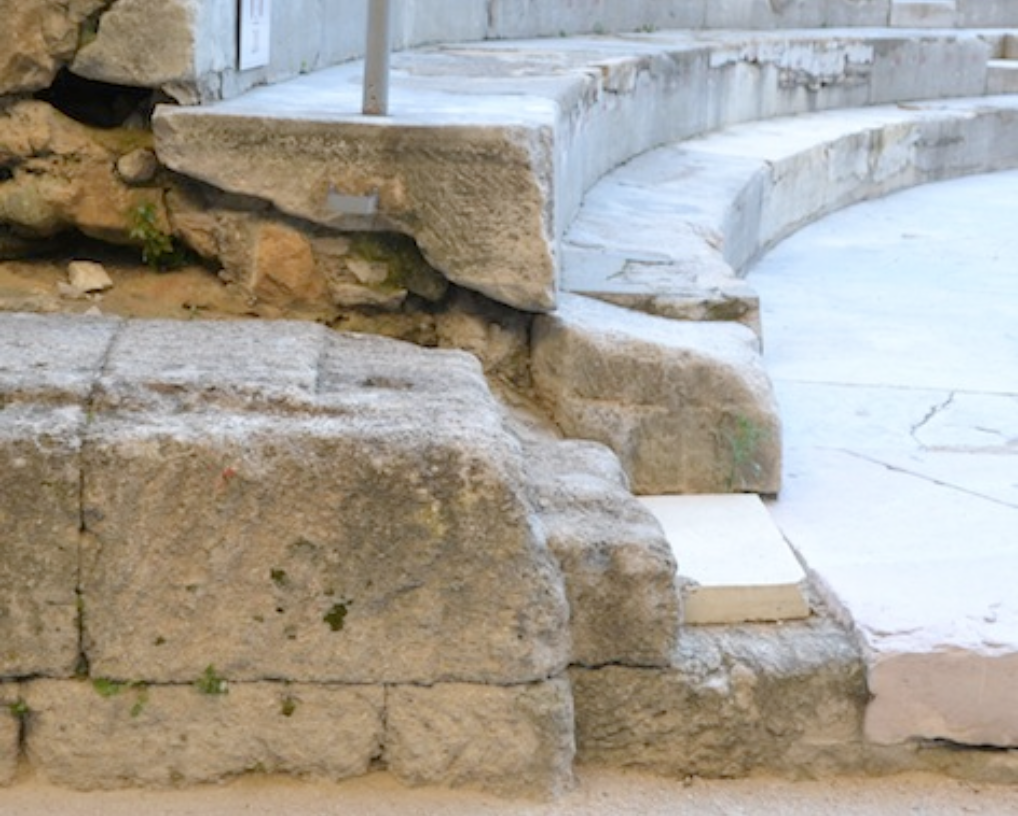
\includegraphics[scale=0.37]{images/gradinCoupe}
		\caption[Repose pied et premier gradin du premier \gls{cuneus}]{Le repose pied et le premier gradin du premier \gls{cuneus} : vu de l'extrémité nord avec au premier plan, le mur bordant l'\gls{aditus} est} 
		\label{coupeGradin} 		
	\end{subfigureth}	
	\qquad
	\begin{subfigureth}{0.49\textwidth}
		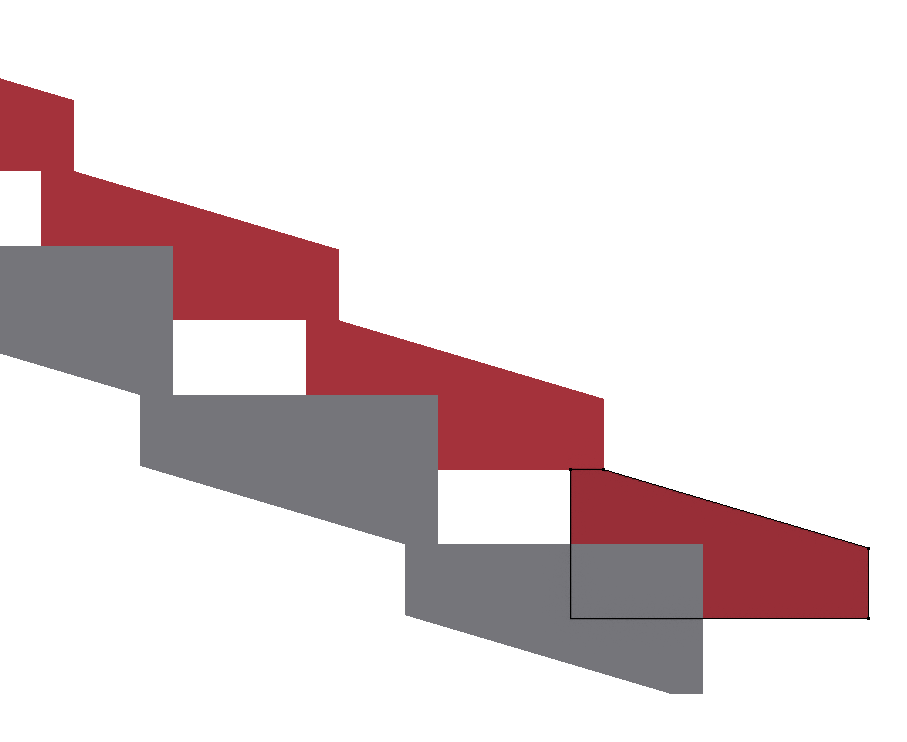
\includegraphics[scale=0.22]{images/escaliers}
		\caption[Modélisation des \gls{maenianum}]{Modélisation des \gls{maenianum} et de l'emprunte des escaliers à retirer après application des modifers Array et Screw}
		\label{modelMaenianum} 		
	\end{subfigureth}	
\end{figure}

En ce qui concerne les escaliers, nous créons d'abord une forme plane de base pour un gradin. Chaque marche mesure la moitié de la hauteur et de la profondeur apparente d'un gradin, et, il s'agit d'en découper le coin extérieur. Pour cela, pour chaque \gls{maenianum}, on crée une copie du gradin de référence (la forme plane sans modificateur) à qui on fait effectuer une rotation de 180° autour de sa normale. On place ensuite le coin extérieur de la copie au centre du gradin (voir fig. \ref{modelMaenianum}) et on la décale de cinq centimètres sur sa longueur. On applique alors à cet "objet escalier" le même \gls{array} que pour les gradins afin de répéter la forme sur toute la hauteur du  \gls{maenianum}. On utilise ensuite un \gls{solidify} pour donner à l'escalier sa largeur. Cette valeur est fixée d'après \cite[Pl. XIX]{orangePl} mais reste modifiable. On utilise à nouveau un \gls{array} pour répéter de manière circulaire les escaliers autour du centre de la \gls{cavea}. On a ainsi cinq escaliers au niveau du premier \gls{maenianum} et neuf au niveau des deuxième et troisième. L'escalier de référence est sur l'axe X (donc en y = 0). Pour le premier \gls{maenianum} on le répète tous les 45°. Pour les deuxième et troisième \glspl{maenianum}, l'escalier de base est répété comme les caissons et les vomitoires, avec un angle de 21,95°, et, en leur faisant faire une rotation de 23,95° par rapport l'origine. Il y a néanmoins une subtilité pour ce qui concerne les marches alignées avec les \gls{parodos}. Pour le premier \gls{maenianum}, ces marches ne sont pas centrées sur l'axe des X, mais décalées de la moitié de leur largeur. Les dix premiers gradins s'arrêtant en $y = 0$, on aurait eu des marches deux fois trop étroites à cet endroit, de même qu'au niveau de la tribune. Pour les modéliser, il suffit de dupliquer l'objet de base utilisé pour soustraire les marches et paramètrer son \gls{solidify} avec un offset de -1 au lieu de 0. Cela permet d'extruder le plan d'un coté uniquement, alors qu'un offset 0 extrude le plan de part et d'autre. On effectue la même démarche pour le repose-pied. Pour les deuxième et troisième \glspl{maenianum}, les traces présentes sur le mur des basiliques indiquent que les escaliers étaient en bordure de gradins. Les marches alignées avec les \gls{parodos} sont donc creusées en utilisant une copie de la forme de base décalée de 3,6m sur l'axe Y. On utilise un \gls{mirror} pour les rendre symétriques par rapport au centre de la \gls{cavea}.
Une fois les \glspl{modifier} appliqués sur les \glspl{maenianum} et le maillage fermé, on peut soustraire les marches d'escaliers à l'aide d'un \gls{boolean}. On soustrait également une marche sur chaque \gls{precinction} de "l'objet cavea". Le premier \gls{maenianum} est également percé, tout comme la \gls{cavea}, au niveau de l'entrée menant au dixième gradin.

		
\section{Les \glspl{aditus} et les tribunes} 

\begin{figure}[!h]
	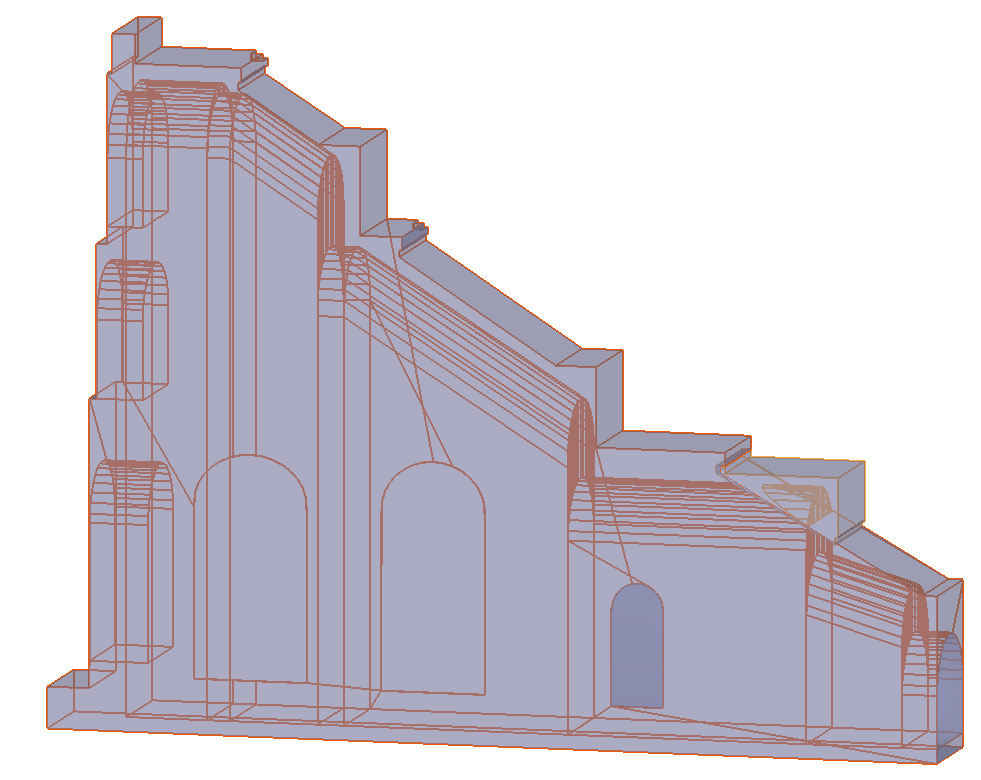
\includegraphics[width=\linewidth]{images/modAditus}
	\caption{Modélisation de l'\gls{aditus} occidental et de sa tribune} 
	\label{modAditus} 
\end{figure}  
		
les \glspl{aditus} sont en réalité une extension de la \gls{cavea} qui se prolonge de manière rectiligne sur l'axe Y (sud-nord). Il est important pour le modèle numérique qu'il y ait jonction entre "l'objet cavea" et les "objets aditus", en tout cas sur la partie commune, c'est à dire, partout excepté au niveau des \gls{parodos}. Or, les relevés (voir fig. \ref{aditusOccidental} et \ref{aditusOriental}) stipulent des mesures qui différents d'un \gls{aditus} à l'autre. Par ailleurs, ces plans donnent également des informations contradictoires avec la coupe théorique de la \gls{cavea} (fig. \ref{coupeCavea}) ayant servie de référence pour la modélisation de "l'objet cavea". Néanmoins, nous avons vu dans la section \ref{La cavea et ses substructures} les différentes causes possibles d'incohérence au niveau des cotes. Il faut donc trancher, et dans un premier temps, nous modélisons les \glspl{aditus} est et ouest de façon à ce qu'ils coïncident avec la \gls{cavea} théorique. Il sera facile dans un deuxième temps d'affiner les cotes de chaque  \gls{aditus} si l'on souhaite que le modèle porte ces informations. On comprend donc qu'il s'agit ici d'un choix de modélisation privilégiant des cotes théoriques, ou en tout cas moyennes, en dépit de cotes exactes relevées en certains points précis. Cela permet d'avoir une \gls{cavea} à un niveau d'élévation parfaitement constant d'une \gls{basilique} à l'autre. 

L'intérieur des \glspl{aditus} est composé d'un enchainement de voutes en berceau permettant le passage sous la \gls{cavea}. Les mesures de ces voutes sont données par la figure \ref{aditusOccidental} pour l'\gls{aditus} occidental, et la figure \ref{aditusOriental} pour l'\gls{aditus} oriental. Un objet à l'est et un objet à l'ouest, épousant la forme de ces voutes, sont créés par extrusions successives, et permettent de creuser les "objets aditus" par \gls{boolean}. Ces voutes sont alignées sur l'axe X (est-ouest) et centrée à 1m80 de l'origine car, la figure \ref{cotes} indique que la partie rectiligne de la \gls{cavea} mesure 3m60. Leur largeur, et donc la largeur des \gls{parodos}, est de 1,52m d'après \cite[Pl. XXI]{orangePl} et en appliquant le règle \ref{epaisseur}. les \glspl{aditus} sont symétrisés à l'identique à l'est et à l'ouest par un \gls{mirror}, mais, les voutes à l'intérieur sont différenciées et modélisées selon les figures \ref{aditusOccidental} et \ref{aditusOriental}. La partie extérieure est modélisées grâce à une copie de l'objet \gls{cavea} que l'on coupe à partir du dixième gradin pour laisser l'espace aux \gls{parodos}. L'objet plan est ensuite épaissi de 3,6m grâce à un \gls{solidify}. Il est important de noter que tant qu'un \gls{modifier} n'est pas appliqué, il est toujours possible de le masquer ou de le modifier. A la différence du \gls{screw}, le \gls{solidify} permet l'utilisation du \gls{boolean} sans avoir besoin de l'appliquer définitivement. Cela laisse une grande flexibilité quand à la modifiabilité du modèle. les \glspl{aditus} sont percés par deux grandes baies à arcature donnant dans les basiliques. Les figures \ref{aditusOccidental} et \ref{aditusOriental} en donne les élévations tandis que leur largeur est donnée par A.Caristie (fig. \ref{caristieDessus}) du coté occidental. Celles-ci seront réutilisées du coté oriental. les \glspl{aditus} sont également percés par la porte (symétrisée en miroir) donnant accès aux tribunes, dont la modélisation est décrite dans la section \ref{sect-escaliers}.

La tribune est modélisée séparément afin de venir s'imbriquer sur l'\gls{aditus}. Elle repose sur le quatorzième gradin et s'élève jusqu'à 48m98, soit environ la moitié du dix-neuvième (voir fig. \ref{aditusOccidental}). Sa bordure donnant vers l'orchestre est alignée avec celle du quinzième gradin. Elle est symétrisée par un \gls{mirror}.

\section{Le mur de scène et ses \glspl{basilique}} 
\label{mur}


\begin{figure}[!h]
	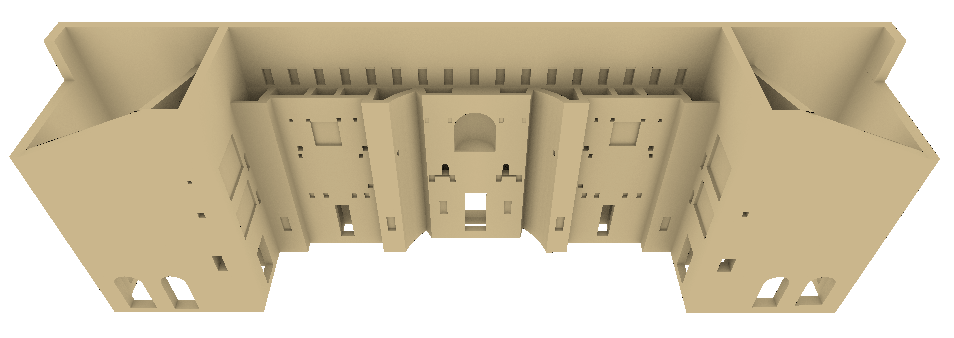
\includegraphics[width=\linewidth]{images/modMur2}
	\caption{Modélisation du \gls{postscaenium} et de ses \glspl{basilique}} 
	\label{modCavea} 
\end{figure} 

Le mur de scène ainsi que ses deux basiliques constituent un bloc distinct. La base est entièrement créée grâce aux cotes de la figure \ref{cotes}. La première étape est de positionner un point aux coordonnées [-51,96 ; 3,52 ; 40] correspondant au point sud-ouest de la base de la basilique ouest. On extrude alors ce point selon les axes X et Y, en respectant les cotes indiquées, afin de tracer la forme extérieure du mur. Les cotes de profondeur de basiliques ne correspondent pas entre la partie orientale et occidentale, on utilise donc la règle \ref{epaisseur} afin de s'assurer que la façade nord soit bien alignée avec l'axe X. Construire un mur tilté aurait grandement compliqué la modélisation sur reste du bâtiment. Lorsqu'une cote n'a pas été spécifiée, on utilise la mise à l'échelle du plan. La seule partie qui n'est pas alignée sur les axes X et Y est l'\gls{exedre} curviligne enclavant la porte royale. Celle-ci est modélisée à partir d'un cercle de 23,5m de diamètre pour lequel on ne garde que six segments à gauche et sept à droite. Cela forme la partie incurvée du mur. Une fois le contour de la base complet, on extrude le plan ainsi obtenu verticalement jusqu'à 76,42m, ce qui correspond à la plus haute élévation du mur.
Sont ensuite crées des objets aux dimensions des pièces et traversant le mur dans toute sa hauteur. A l'aide d'un \gls{boolean} ces objets sont soustraits à la forme de base. On note quelques valeurs aberrantes sur le plan de \cite[Pl. XXI]{orangePl}, surement dues à des erreurs de recopie, et qui sont à présent corrigées dans le modèle numérique. 

La même méthode est utilisée pour découper le haut du mur qui supportait le toit. On s'appuie alors sur la restitution de A.Caristie (voir fig. \ref{toitCaristie} et \ref{toitBadie}) qui propose, pour la partie sommitale du front de scène, une taille en biseau permettant de soutenir les poutres de la couverture de scène. Cet angle de 19,25° est aligné avec les traces que la couverture a laissé sur le mur, et coupe l'intégralité du sommet du \gls{postscaenium}. On notera que la modélisation nécessite une valeur d'angle plus précise que celle du rapport de l'\gls{iraa} \cite[fig. 24]{orangeTxt} de 19°. On creuse également la façade sud du mur nord avec un "objet poutre", dont la modélisation est expliquée dans la section \ref{sect-couverture}, afin de créer les trous d'encastrement. La partie sommitale des \glspl{basilique} est également découpée en soustrayant un objet dont la forme est dessinée selon la méthode suivante : 
Ayant plus d'information sur la basilique occidentale que sur l'orientale, la même forme sera reproduite en miroir pour les deux basiliques et on appliquera le modifier pour pouvoir modifier les cotes qui différents. Avec de nouvelles informations il sera par la suite facile pour les archéologues d'affiner les autres cotes de la partie orientale en corrigeant cet objet. Le sommet des murs est et ouest des \glspl{basilique} se présente horizontalement tout comme la partie au dessus des \glspl{parascaenium}. Nous les plaçons selon les élévations des figures \ref{aditusOccidental} et \ref{aditusOriental}. Sur le mur sud, ces deux parties se rejoignent avec une pente de 21°. On laissera le mur nord revenir sur les flancs extérieurs sur 4,3m \cite[p. 38]{orangeTxt}. Pour créer la pente sommitale du mur séparant la \gls{basilique} avec la cage d'escalier, on utilise la figure \ref{grenier}. Ce mur soutenait la charpente de la couverture. On constate à ce stade un problème d'incohérence avec le plan \ref{cotes} qui indique, comme longueur de mur, 15m44. En appliquant l'échelle de la figure \ref{grenier}, on obtient 16m de longueur. Ce plan a pourtant l'air correct car les dimensions de la porte donnant dans les combles correspond bien à celles indiquées dans le rapport. On comprend alors que l'épaisseur des murs diminue avec la hauteur. Cet amincissement s'opère à priori au moment des changements d'ordre, et parait logique d'un point de vue architecturale. Effectivement, les parties hautes sont souvent plus fines que les parties basses afin d'alléger la charge et améliorer la portance. Il suffit donc d'augmenter la longueur des salles des \glspl{basilique} au niveau du troisième ordre pour obtenir la bonne cote. N'ayant pas d'information précise sur l'épaisseur des murs entre les combles et la base du théâtre, nous conservons les cotes initiales pour le reste du bâtiment. Néanmoins, ces données pourront être affinées par la suite.

Pour réaliser les 17 portes donnant sur la \gls{porticus ps}, on utilise également le plan \ref{cotes}, en réalisant une mise à l'échelle lorsque les valeurs numériques de largeur ne sont pas indiquées. La modélisation de leurs élévations n'est malheureusement pas très précise car, faute de valeur numérique, celles-ci sont estimées grâce aux dessins de H.Daumet \cite[Pl. XII, XIII, XIV]{orangePl}. On note que certaines portes arrivent à l'affleurements des pièces du \gls{postscaenium}, or, les \gls{boolean} se comportent mal lorsque deux faces sont superposées entre l'objet soustrait et l'objet à soustraire. Pour résoudre ce problème, on décale la porte de quelques millimètres, ce qui créera une légère saillie sur le mur, mais qui pourra être corrigée une fois le modifier appliqué. A l'intérieur du \gls{postscaenium} se trouvent également des passages permettant d'accéder d'une pièce à l'autre pour chaque étage. On utilise les figures \ref{1erniveau}, \ref{2emeniveau} et \ref{3emeniveau} pour les placer dans le plan XY et on les positionne en élévation au niveau du bas du \gls{podium} de chaque ordre. Leur forme est donnée par A.Caristie \cite[Pl. II]{orangePl}

La façade du front de scène possède elle aussi des trous d'encastrement ayant pour leur part servis à accrocher la décoration. Ceux-ci sont créés à l'aide d'un \gls{boolean} en respectant les mesures d'élévation du plan \ref{frontdescene}. Sur cette même façade sont également percées les trois portes traversant le \gls{postscaenium} ainsi que les différentes niches représentées sur ce plan. Tous ces objets sont modélisés par mise à l'échelle des plans \cite{orangePl} ou grâce aux valeurs numériques indiquées dans le rapport \cite[Chap. II]{orangeTxt}. Ils sont symétrisés par rapport à la porte royale. Effectivement, les informations recueillies concernent principalement la partie occidentale et ne reflètent que l'état actuel du mur. L'érosion des arrêtes fausse donc de toute façon une éventuelle restitution exacte. L'étude de ces encastrements ne peut donc être décorrélée de la restitution globale du décor du front de scène (voir \ref{sect-autres}). De part et d'autre de la porte royale se trouvent deux niches créées par la soustraction d'un demi-cylindre verticale. Au-dessus, à la frontière avec le second ordre se trouvent de petites baies à arcature. Encore au dessus, et centré sur le front de scène, se trouve une grande niche abritant aujourd'hui une statue dite d'Auguste. Cette niche est l'emprunte d'un demi-cylindre vertical dont la face supérieur est un demi-cylindre horizontal. L'assemblage se fait en faisant la différence de ces deux objets et en pointant les normales du demi-cylindre du haut vers l'extérieur. Au dessus des portes latérales du front de scène et au niveau du troisième ordre se trouvent deux niches que l'on creuse dans le mur sur la moitié de son épaisseur. Cela correspond également à la profondeur de la porte d'après le plan \ref{cotes}. Leur emplacement est déterminé par le plan \ref{frontdescene}. En considérant ces deux plans ainsi que le relevé \ref{retourmur}, on crée, sur les murs de retour, les portes donnant accès aux \gls{parascaenium}, les niches, ainsi que les ouvertures qui permettaient vraisemblablement à l'époque l'apparition de personnages sur des balcons. De la même manière on produit trois ouvertures rectangulaires sur la façade sud de la \gls{basilique} ouest (voir fig. \ref{aditusOccidental}) et deux sur la \gls{basilique} est (voir fig. \ref{aditusOriental}). L'ouverture la plus basse est une porte menant de la première \glspl{precinction} au premier étage des \glspl{basilique}.


\section{Le \gls{pulpitum} et l'\gls{orchestra}} 

\begin{figure}[!h]
	\includegraphics[width=\linewidth]{images/modOrchestre}
	\caption[Modélisation de la scène, l'\gls{orchestra} et le sol des \gls{parodos}]{Modélisation de la scène (marron), l'\gls{orchestra} (vert) et le sol des \gls{parodos} (gris)} 
	\label{modOrchestre} 
\end{figure} 

Le \gls{pulpitum}, autrement dit l'estrade de scène, a aujourd'hui complètement disparu et a été remplacé par un plancher moderne. Il reste néanmoins des traces sur le mur de scène qui permettent de s'approcher de sa version antique. Les figures \ref{aditusOccidental} et \ref{aditusOriental} donnent les élévations du pulpitum ainsi que de l'orchestre sur les extrémités orientales et occidentales. Ces mêmes plans donnent aussi les niveaux du sol des \glspl{parodos}. Nous créons donc un objet selon ces élévations. La différence étant notable à l'est ou à l'ouest, l'objet n'est pas symétrisé mais bien singularisé de chaque coté. La face inférieure termine au même niveau d'élévation que l'orchestre pour faire jonction. Entre les deux \glspl{aditus}, le front du \gls{pulpitum} était ornée d'une frise de 75cm d'épaisseur terminant a ses extrémités par deux escaliers de quatre marches et larges de 89cm \cite[p. 458]{formigeBis}. La frise est ainsi créée par extrusion et les escalier par d'opération de différence à l'aide d'un \gls{boolean}.

L'orchestre est une forme volumique dont la face supérieure représente le sol. Il pourra être, dans une prochaine étape, creusé à l'aide de \gls{boolean} pour réaliser l'\gls{hyposcaenium} et le caniveau \cite[Chap. VI]{orangeTxt}. Cet objet sert également de sol à l'intérieur des \glspl{basilique}. De la même manière que la couverture du caniveau (voir \ref{La cavea et ses substructures}) nous créons le \gls{balteus} d'après les relevés de A.Carisite \cite[Pl. I]{orangePl}. Son épaisseur est fixée à 13cm conformément aux éléments encore visible en bordure de la moitié orientale de l'\gls{orchestra} \cite[p. 340]{orangeTxt}. Sa hauteur est fixée à 1m50 comme celui du théâtre antique de Sabratha \cite[p. 96]{lachaux} est n'a donc qu'un rôle purement illustratif.

\section{Les couvertures du bâtiment de scène}
\label{sect-couverture}

\begin{figure}[!h]
	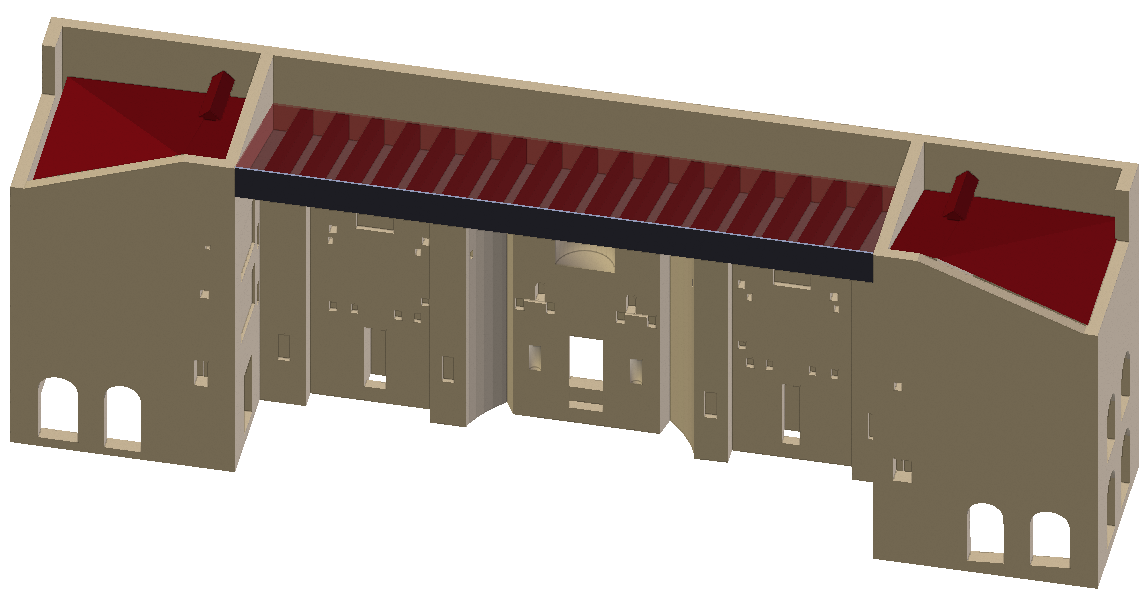
\includegraphics[width=\linewidth]{images/modCouvertures}
	\caption{Modélisation des couvertures de scène et des basiliques} 
	\label{modCouvertures} 
\end{figure} 
Nous avons expliqué dans la section \ref{couverture} quelles sont les hypothèses de restitution de la couverture du \gls{pulpitum} et avons vu que plusieurs propositions existent. Nous en avons choisi une, à implémenter dans le modèle, sans toute fois entrer dans une étude de construction architecturale. Nous modélisons donc l'hypothèse de toiture parallélépipédique \cite[Chap. I, sect. 6]{orangeTxt}, qui remet en question celle de A.Caristie de forme triangulaire (voir fig. \ref{toitCaristie} et \ref{toitBadie}). Nous créons donc, dans le plan YZ, un parallélogramme incliné à 19,25°, épousant l'emprunte dans le mur donnée par la figure \ref{toitBadie}. Cette forme plane est placée à 27,25m du centre sur l'axe X pour correspondre à la figure \ref{frontdescene}. En utilisant un \gls{solidify} sur 1,2m nous créons la largeur de la poutre. Cette largeur est une moyenne approximative déterminée d'après les trous d'encastrement actuellement visibles. Ceux-ci ayant subi de nombreuses altérations, il est très difficile de déterminer une largeur exacte sans une étude approfondie du sujet. L'\gls{iraa} explique d'ailleurs que plusieurs toitures différentes auraient été testées, voire utilisées, durant le vie du théâtre et qu'il n'y a donc pas une unique solution \cite[p. 34]{orangeTxt}. Néanmoins, une simple modification du paramètre de largeur permettra de tester facilement les différentes hypothèses. Cette poutre est alors répétée dix-sept fois avec un espacement de 2,83m par un \gls{array} (espacement moyen estimé pour les mêmes raisons que les largeurs). Nous créons ensuite un nouvel objet composé de trois plans de quelques centimètres d'épaisseur, allant d'une basilique à l'autre, et encapsulant les poutres par le dessus, le dessous et le l'avant. Le plan de devant est vertical et simule l'emplacement d'une frise décorant la devanture du toit. Les deux autres simulent respectivement le dessus et le dessous de la toiture.

Nous avons vu dans la section \ref{mur} comment a été modélisé le sommet des \glspl{basilique} et quelles en étaient les cotes. Nous reprenons donc ces valeurs pour modéliser la couverture de cette partie du bâtiment. On utilise uniquement des objets plans car l'aspect volumique ne nous intéresse pas à ce stage de l'étude. Seule la forme et la présence de cet objet nous est utile et celui-ci pourra être améliorer par la suite par des experts charpentiers. La structure se compose d'une partie plate inclinée à 21° (comme le mur la soutenant) couvrant le \gls{parascaenium} et la cage d'escalier et d'un plan, couvrant la \gls{basilique}, coupé en deux triangles, représentant l'\gls{aretier} (voir section \ref{couverture-basi}). L'\gls{iraa} décrit la présence d'un "petit toit à double pente" \cite[p. 34]{orangeTxt} au dessus de la cage d'escalier permettant de monter sur le toit. Celui-ci est modélisé à titre démonstratif mais trop peu d'informations sont disponibles pour nous permettre d'utiliser des cotes précises.


\section{La \gls{porticus isc}}

\begin{figure}[!h]
	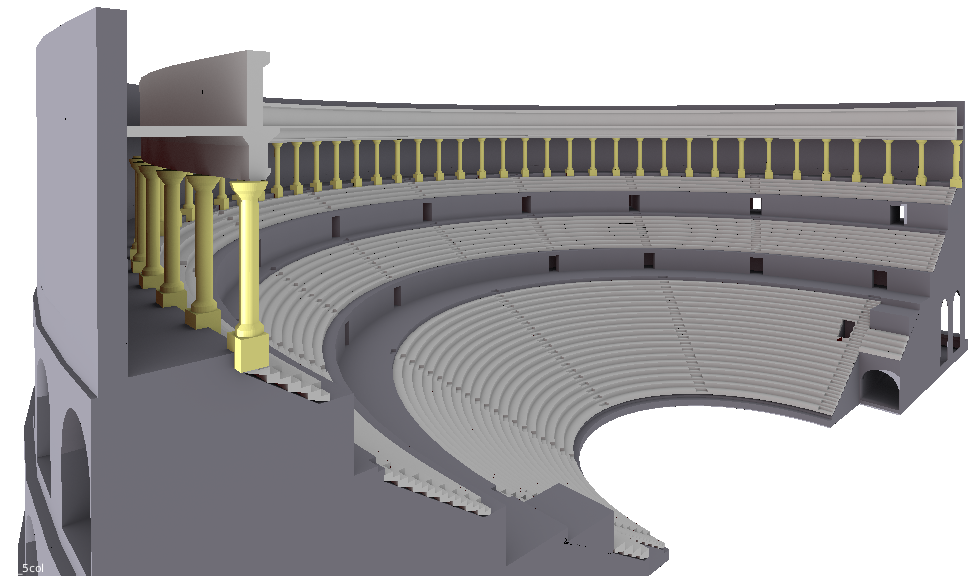
\includegraphics[width=\linewidth]{images/modPorticus}
	\caption{Modélisation de la \gls{porticus isc}} 
	\label{modPorticus} 
\end{figure} 

Au dessus du troisième \gls{maenianum} se trouvait une \gls{porticus isc} faisant tout le tour de la \gls{cavea}. La première colonne était encastrée sur la moitié de sa largeur dans le mur de la basilique. C'est d'ailleurs grâce à cela que l'on peut connaitre ses dimensions. On sait par ailleurs que l'entrecolonnement d'un portique était constant et précis dans les théâtres romains. On crée donc la première colonne avec une forme géométrique grossière correspondant au dessin de A.Caristie (fig. \ref{colonneCaristie}) que l'on duplique en miroir. Ces deux colonnes sont créées séparément car elles sont au dessus des \glspl{aditus}, donc en dehors du cercle formé par la \gls{cavea}. On va ensuite créer le reste des colonnes circulairement autour de la \gls{cavea} comme nous l'avons fait pour les caissons soutenant le troisième \gls{maenianum} (voir \ref{La cavea et ses substructures}). Or, on se pose la question du nombre de colonnes qu'il y a en tout. A.Caristie suppose qu'il y en 34, c'est à dire cinq pour les \gls{cuneus} aux extrémités de la \gls{cavea} et quatre aux autres. On prend comme hypothèse que les escaliers arrivent toujours à égale distance de deux colonnes successives. On mesure entre la première colonne et l'escalier E13 (voir \ref{2emeniveau}) un angle de 28,35°. Cet angle correspond à $n+0,5$ fois l'entrecolonnement que l'on cherche. Dans l'hypothèse de A.Caristie, il y a quatre colonnes par \gls{cuneus}, plus une encastrée. Sur le rapport de l'\gls{iraa} \cite[Pl. XX]{orangePl} il y en à quatre aussi pour les six \gls{cuneus} centraux et deux de plus pour les \gls{cuneus} latéraux. On remarque que dans ce dessin, l'entrecolonnement n'est pas régulier, ce qui est contraire à nos hypothèses de modélisation. On va donc chercher le nombre de colonnes nécessaires pour répondre à nos conditions avec une, deux ou trois colonnes supplémentaires sur les \gls{cuneus} latéraux. On résout alors le système d'équation suivant :


\begin{equation}
  \left \{
   \begin{array}{r c l}
      \alpha \times n_{Col}  & = & 21,95 \\
      \alpha \times (n_{Col} + n_{Sup} - 0,5)   & = &  28,35
   \end{array}
   \right .
\end{equation}

Avec : \\
$\alpha$ : l'angle décrit entre deux colonnes \\
$n_{Col}$ : le nombre de colonnes dans les cuneus centraux \\
$n_{Sup}$ : le nombre de colonnes en plus dans les cuneus latéraux \\

On obtient : \\
$n_{Sup}$ = 1 $\Rightarrow$ $\alpha$ = 12,8° et $n_{Col}$ = 1,7 \\
$n_{Sup}$ = 2 $\Rightarrow$ $\alpha$ = 4,7° et $n_{Col}$ = 5,14 \\
$n_{Sup}$ = 3 $\Rightarrow$ $\alpha$ = 2,56° et $n_{Col}$ = 8,57 \\


Ces résultats montrent que l'agencement le plus probable est d'avoir cinq colonnes par \gls{cuneus} et deux de plus pour les extrémités de la \gls{cavea}. On ne tombe cependant pas sur un chiffre rond mais on peut estimer que cette erreur de 0,14° est négligeable sur l'ensemble de la structure. Dans le modèle, nous positionnons donc une colonne en $y=0$ et en $x=-46,78m$ (distance correspondant à la troisième \gls{precinction}). Celle-ci est répétée 42 fois pour atteindre 180° et se retrouver en symétrique de l'autre coté de la \gls{cavea}. On utilise pour cela un \gls{array} avec un angle de 4,39°, soit $180°/41$. On obtient donc un entrecolonnement de :
\begin{equation}
	\frac{l}{2} =  46,78 \times  sin(\frac{180}{2 \times 41}) 
\end{equation}
\begin{center}
	soit $l = 3,58m$
\end{center}	

La première colonne, et son symétrique, sont encastrées de moitié dans le mur de la basilique en $y=3,6m$, ce qui nous donne bien un entrecolonnement régulier sur l'ensemble de la \gls{porticus isc}. Sa couverture est modélisée à partir de la représentation de A.Caristie \cite[Pl. III et VI]{orangePl} puis extrudée à l'aide d'un \gls{screw} autour de la  \gls{cavea}. Elle est dupliquée et étendue au dessus des \glspl{aditus} à l'aide d'un \gls{solidify} couplé à un \gls{mirror}. On constate sur la figure \ref{modPorticus} que les vomitoires séparent bien les colonnes du portique par groupe de cinq et qu'il en reste deux au dessus des  \gls{aditus}.

\section{Les escaliers} \label{sect-escaliers}

\subsection{Accès aux tribunes par les  \gls{aditus}}

\`A l'est et à l'ouest, depuis l'intérieur des  \gls{aditus}, certains spectateurs privilégiés avaient accès aux tribunes par un escalier menant à la moitié de l'\gls{ima cavea}. Ceux-ci n'ont pas été restaurés mais le plafond vouté est néanmoins visible aujourd'hui (voir fig. \ref{parodos}). Pour modéliser cet escalier, on sait que la première marche commence à 41,11m d'altitude et la dernière arrive à 45,58m. Or celui-ci débouchait probablement au dixième gradin, là où la partie basse de la  \gls{cavea} s'arrête et où la partie haute est soutenue par l'\gls{aditus}. On a donc 20 marches d'une hauteur de 22,35cm. \`{A} partir de la première marche, que l'on ajuste en longueur, et à l'aide d'un \gls{array}, on complète l'escalier pour arriver au dixième gradin. On perce alors la \gls{cavea} avec un objet représentant l'ouverture dans les gradins. A compléter ...

\begin{figure}[!h]
	\centering
	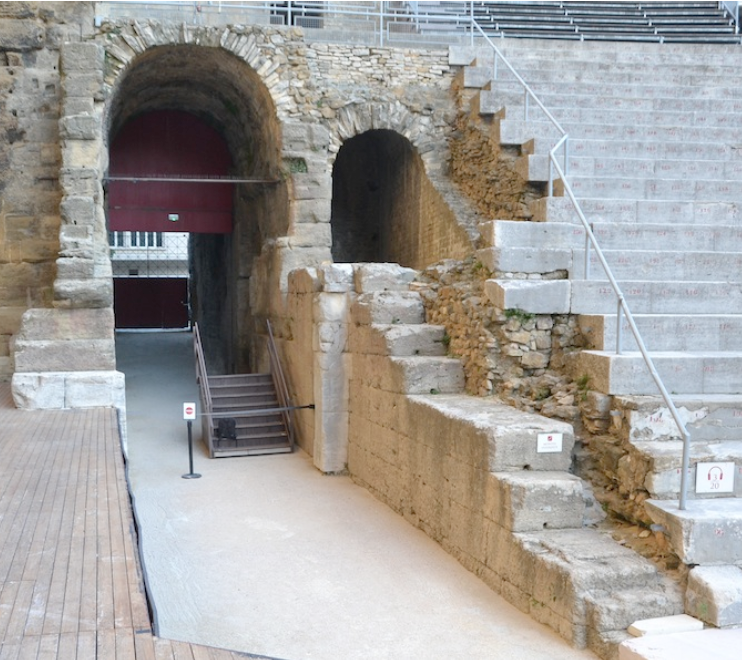
\includegraphics[width=0.5\textwidth]{images/parodos}
	\caption[\Gls{parodos} oriental et entrée menant à l' \gls{ima cavea}]{\Gls{parodos} oriental et entrée menant à l' \gls{ima cavea} \footnotemark} 
	\label{parodos} 
\end{figure}
 \citefnt[fig. 418]{orangeTxt}

\subsection{Accès à la  \gls{cavea} depuis l'extérieur}

\subsection{Les cages escaliers des \gls{parascaenium} et les paliers internes}


On place également en haut des basiliques un plancher supporté par six poutres qui faisait office de combles. Les trous d'encastrement supposent des poutres alignées sur l'axe est-ouest de largeur : 55cm, de hauteur 48cm et enfoncées de 48cm en moyenne. Nous en modélisons une que nous plaçons à l'aide du plan \ref{grenier} et que nous répétons six fois avec un \gls{array} avec une espacement de 4,18m. Cette structure sera dupliquée pour créer les deux autres paliers de la basilique. Leurs élévations sont données par ... explication des escaliers

\subsection{Les escaliers extérieurs}

Section à reprendre ...

\`{A} l'est et à l'ouest, la première porte d'arcades après l'\gls{aditus} donnait sur un escalier permettant d'accéder au premier \gls{ambulacre}. L'escalier oriental (fig. 435) a été restauré avec 31 marches par J.-C. Formigé, qui l'a fait aboutir dans l'\gls{ambulacre} à un niveau de sol séparé par 4 marches de celui de la première  \gls{precinction}. A. Caristie restituait un escalier de 24 marches conduisant à un premier \gls{ambulacre}, dont le niveau de sol aurait été beaucoup plus bas que celui de la première  \gls{precinction} (pl. VI). Une dizaine de
marches aurait permis d'aller de l'\gls{ambulacre} à la  \gls{precinction}.
Du côté ouest, J.-C. Formigé a restauré un escalier de 32 marches conduisant à
l'\gls{ambulacre} (fig. 428)


\section{La colline Saint-Eutrope} 
La colline Saint-Eurtope, qui soutient le théâtre sur sa partie méridionale, a été modélisée d'après les lignes d'altitude représentées sur la figure \ref{colline}. On commence par créer la ligne la plus basse que l'on trace point par point pour faire une face de base. Celle-ci sera alors extrudée vers le haut six mètres par six mètres. Tranche par tranche, on ajuste les points pour coller au plan. Seule la partie soutenant le théâtre nous intéresse, la partie sud de la colline se termine donc simplement en reliant les points du flanc ouest et est. Les élévations ont ensuite été légèrement adaptées tranche par tranche pour s'encastrer au mieux dans le théâtre. La colline est donc actuellement peu précise et il est nécessaire de l'affiner à l'aide d'un document détaillant mieux sa géométrie. Il sera notamment appreciable d'affiner précisément la partie soutenant le théâtre ce qui risque d'être difficile de par la non accessibilité du terrain. Le plus important est d'être précis sur la substructure de la  \gls{cavea} en plaçant les murs séparant les  \glspl{ambulacre} de la colline précisément. Effectivement la roche naturelle n'était pas apparente à l'intérieur du théâtre. Elle l'est aujourd'hui par endroit, notamment dans les pièces de type "grotte" du premier \gls{ambulacre}, mais celles-ci ne sont pas d'origine. On utilise un effet "\textit{smooth}" pour lisser les arrêtes et rendre l'aspect plus naturel.

		
		
		
		
		
		
		
		
		
		
		
\chapter{Applications}
	\citationChap{
	Imagination is as effortless as perception, unless we think it might be ‘wrong’, which is what our education encourages us to believe.
	}{Keith Johnstone}
	\minitoc
	\newpage

\section{Introduction}
Le modèle numérique décrit dans la partie précédente tend à restituer de manière simplifiée le théâtre d'Orange dans sa version d'origine. Le maillage n'est fait que de formes géométriques simples, c'est à dire avec un niveau de détail ne descendant pas en dessous de la dizaine de centimètres. Les cotes sont par contre précises lorsqu'elles proviennent d'un plan référencé. Mais il est important de noter que ce projet s'inclut dans une thématique plus vaste de restitution du théâtre antique d'Orange. Son essence est donc de permettre l'incorporation de nouveaux résultats de recherche. Cette partie a pour but de présenter le potentiel d'une telle maquette en terme d'applications. Nous verrons les différentes implémentations architecturales ou graphiques qui permettent de réaliser des simulations statiques ou dynamiques.

\section{Le \gls{velum}} \label{sect_velum}

Il existe de nombreuses théories sur la disposition des \glspl{velum} des théâtres romains et pour cause, il en reste très peu de trace. Seules quelques documentations d'origine  décrivent approximativement cette toile protégeant le public du soleil. Nous choisissons donc d'adopter la représentation de A.Caristie \cite[Pl. VI]{orangePl} qui, bien qu'hypothétique, est une source toute aussi vraisemblable que les autres. On s'intéresse d'abord aux consoles soutenant les mats sur la face nord du bâtiment de scène. Pour les positionner, on utilise la représentation de la façade nord de A.Caristie \cite[Pl. III]{orangePl} en créant une console centrée en haut du mur reproduite 21 fois horizontalement et une fois verticalement. On note que leur espacement est de 1m91. Ces deux séries sont ensuite symétrisées par un \gls{mirror}. On ajoute une dernière paire de console en bord de mur symétrisée de la même manière. Les élévations ne sont pas parfaitement connues, c'est pourquoi on utilise la mise à l'échelle du plan de A.Caristie. Leur forme est rectangulaire et pourra par la suite être dessinée d'après leur forme réelle. Comme expliquée dans la section \ref{sect_postscaenium}, seules douze de ces consoles pouvaient accueillir un mât. Néanmoins, 41 mâts sont modélisés afin de percer les consoles du haut et réaliser la mortaise dans celles du bas. Ceux-ci, de forme cylindrique, se terminent dans la partie basse par une fine tige permettant de percer le trou d'évacuation d'eau. Ces mâts sont répétés grâce à un \gls{array} et seront soustrait aux consoles par un \gls{boolean}. Ils ne servent qu'à cette fonction et seront cachés par la suite. On laissera par contre apparaitre un nouvel objet similaire, comportant les six mâts, se trouvant aux positions où les bouches d'eau sont percées. 

Sur sa représentation du \gls{velum} en vue du dessus  (fig. \ref{velumCaristie}), A.Caristie ne représente que 39 consoles sur le mur arrière au lieu de 43, ce qui rend ce dessin peu fiable. Néanmoins, nous utiliserons ce concept d'anneau central en fer à cheval que nous modélisons de manière fidèle à sa représentation. L'objet de référence est également muni de deux longs et fins cylindres représentant des cordages et reliant les mâts à deux boucles au bout du fer à cheval.
Tout autour de la \gls{cavea} se trouvent également deux séries de consoles fixées au mur arrière de la \gls{porticus isc}. L'agencement le plus crédible est représenté sur le dessin de la face est \cite[Pl. IV]{orangePl}, c'est à dire, un jeu de deux consoles entre chaque \gls{pilastre} du mur extérieur. Il y aura donc deux fois plus de mâts que de triplets d'arcades autour de la \gls{cavea} (voir section \ref{La cavea et ses substructures}). Nous avions 31 arcades, on peut donc placer 62 mâts et leur paire de consoles respective. Il y a deux mâts de part et d'autre au niveau des \glspl{aditus}, il y en aura donc 58 à repartir autour de la \gls{cavea}. Pour déterminer l'angle, on se base sur les 31 arcades précédemment modélisées. On utilise la moitié de leur angle, c'est à dire 3,06°. L'angle total formé par ces 58 mâts est de 174,42°, il faudra donc effectuer une rotation de l'ensemble de 2,79°. L'objet de référence se composant d'une paire de consoles, d'un mât et d'un cordage reliant l'anneau centrale, est placé en $y=0$ et $x=-51,64m$. Pour placer les consoles de l' \gls{aditus} on calcule l'espacement entre les mâts :
\begin{equation}
	l =  51,64 \times sin(3,06) 
\end{equation}
\begin{center}
	soit $l = 2,76m$.
\end{center}

Le premier mât situé sur la partie circulaire de la \gls{cavea} ayant subit une rotation de 2,79° autour de l'axe vertical, on calcule la position du mât de référence pour les  \gls{aditus} :
\begin{equation}
	\begin{array}{r c l}
		l & = & 51,64 \times sin(2,79) \\
		l &= & 2,51m
	\end{array}
\end{equation}
\begin{center}
	donc $y = 0,25m$.
\end{center}

On utilisera ensuite un \gls{array} pour répéter une fois l'ensemble mât-consoles-cordes avec une distance de 2,76m et un \gls{mirror} pour le symétriser à l'est. Encore une fois, on constate que la modélisation contredit les dessins de A.Caristie qui représentaient 67 mâts autour de la \gls{cavea}. On comprend donc que son intention sur ce type de représentations était plus une étude de principe qu'une restitution vraissemblable.

En ce qui concerne l'élévation des mâts, on constate que ceux situé sur le \gls{postscaenium} sont à priori plus haut que ceux autour de la \gls{cavea}. C'est en tout cas ce que suppose les restitutions qui estiment le haut du mur de scène à 76,42m et le mur aval de la rue périphérique à 70,59m \cite[Pl. XLVIII et XLIX]{orangePl}. Il semble en effet cohérent que ce mur continu dans le prolongement des \glspl{basilique}. Selon l'hypothèse de A.Caristie (fig. \ref{velum2}) où le \gls{velum} serait un arceau de la taille de l'orchestre maintenu par des cordages tendus, nous pouvons calculer la hauteur des mâts afin que les cordages arrivent à l'affleurement du toit. Pour cela, considérons que les cordes sont parfaitement tendue et que le cordage arrive également à l'affleurement du mur de la mur périphérique (fig. \ref{dessinvelum}. D'après le théorème de Thales, on obtient :

\begin{equation}
	\begin{array}{r c l}
		h & = & \frac{18,4\times(76,42-70,59)}{51,6} \\
		h & = & 2, 08m
	\end{array}
\end{equation}

Les mâts du \gls{postscaenium} dépasseront donc d'au moins deux mètres pour s'assurer que les cordages ne soient pas en contact avec le toit. Cette hauteur pourra diminuer si les cordages du mur périphérique sont accrochés plus haut. Si h est la hauteur de l'accroche des cordages au dessus du mur périphèrique alors, la hauteur de l'accroche des cordages du \gls{postscaenium} sera de :

\begin{equation}
	\begin{array}{r c l}
		h' & = & 2,08 - \frac{18,4}{51,6} \\
		h' & = & 2, 08 - 0,36 \times h
	\end{array}
\end{equation}

Par exemple si les cordages du mur périphérique sont à 1m au dessus du mur ceux du \gls{postscaenium} seront à 1,72m au dessus du mur. Cela dit, nous sommes dans une situation où les cordages sont parfaitement tendus, or dans la pratique le poids global du velum va entrainer une courbure qui imposera de surélever les accroches des cordages. Nous avons donc calculé ici une hauteur minimum. 
 \begin{figureth}
	\begin{subfigureth}{0.49\textwidth}
		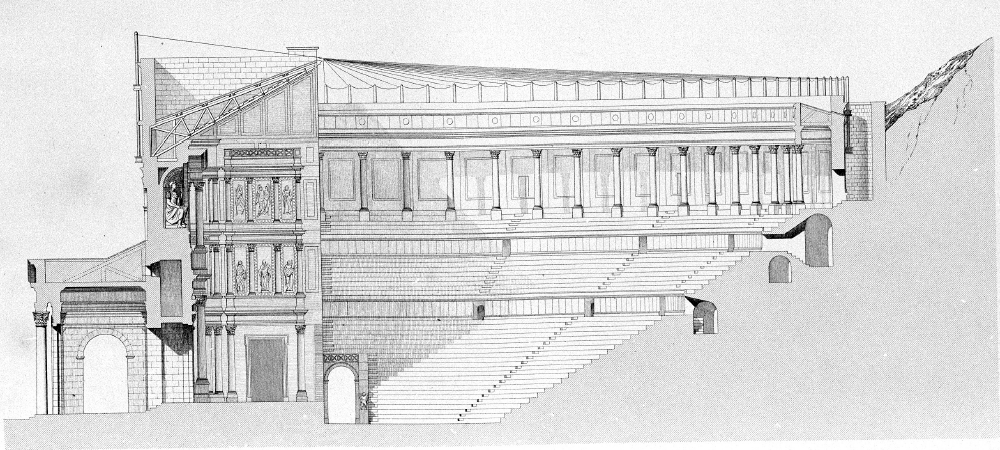
\includegraphics[width=\linewidth]{images/velum2}
	\caption[Coupe axiale vers l'est par A.Caristie]{Coupe axiale vers l'est par A.Caristie \footnotemark} 
	\label{velum2} 
	\end{subfigureth}	
	%\qquad
	\begin{subfigureth}{0.49\textwidth}
		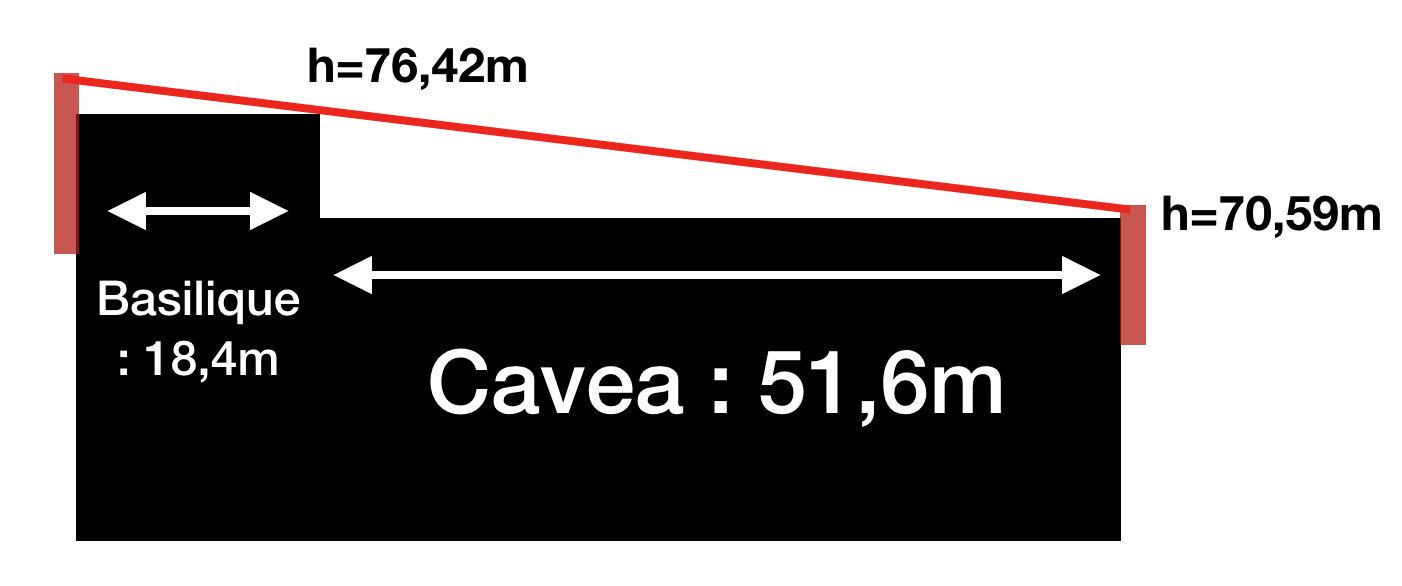
\includegraphics[width=\linewidth]{images/dessinvelum}
		\caption{Schéma de l'angle du velum}
		\label{dessinvelum} 		
	\end{subfigureth}	
\end{figureth}
 \citefnt[Pl. V]{orangePl}

Pour modéliser le voilage située au dessus de la \gls{cavea}, nous allons dans une première étape uniquement placer des objets plans entre chaque cordages. Il suffit pour cela d'utiliser une des arrêtes de la corde pour créer un nouvel objet comportant les mêmes propriétés (centre et \glspl{modifier}). Il suffit ensuite d'utiliser un \gls{screw} pour étendre le plan entre les deux cordages sur 2,79°, ou moins, si l'on souhaite laisser du jour avant le prochaine cordage. On peut également tourner l'arrête de référence ou changer le nombre de répétitions afin d'ombrager une partie ou l'autre de la \gls{cavea}. Grâce à cela nous pouvons tester l'ensoleillement du théâtre et le nombre de voiles à déplier pour abriter les spectateurs. Nous utilisons pour cela un objet "Lamp" de type "soleil" qui émet une lumière depuis l'infini dans une direction choisie. On réalise ainsi l'animation d'une journée du levé au couché du soleil et on analyse selon l'angle au zénith la façon dont les \glspl{velum} devaient être déployés.


Dans un deuxième temps on peut simuler l'ouverture et la fermeture réaliste des toiles en leur affectant une propriété physique de type "cloth". Il faut pour cela créer des toiles rectangulaires de largeur 2m76 et les subdiviser en un nombre important de petits rectangles. On peut alors sélectionner sur le bord des toiles des points qui resteront accrochés aux cordes (en pratique il y aurait des anneaux pour faire coulisser les toiles sur les cordes). On place alors ces points en position "velum déployé" puis "velum rentré", leur affectant à chaque fois une \gls{keyframe} pour réaliser l'animation. Lorsque l'outil physique est appliqué, la toile subit l'effet de la gravité et se plie avec une résolution correspondant à la subdivision effectuée précédemment. On peut alors lancer l'animation pour voir le \gls{velum} se déplier. En utilisant l'option de \gls{baking}, on peut passer l'animation à l'endroit et à l'envers sans avoir besoin de refaire un rendu.

\section{Le rideau de scène}


\section{Les systèmes de \glspl{particule}}
\subsection{Les spectateurs}
Une fois le théâtre modélisé, nous pouvons ajouter des spectateurs dans les gradins. Ceux-ci sont fixes dans un premier temps mais pourraient être animés lors de visualisations vidéo. La modélisation des personnages ne sera pas décrite dans ce document, néanmoins, on peut noter que différent types de spectateur pourraient être modélisés car le placement dans le théâtre dépendait de la classe sociale.

Pour représenter un type de personnage il faut le prendre comme objet de référence et le placer dans une posItion assise à l'aide d'\glspl{armature}. Il faudra ensuite créer un nouvel objet correspondant au bord des gradins afin que les personnages soient bien positionner sur ceux-ci. Cet objet est subdivisé plusieurs fois, puis l'outil d'élimination de double vertices est utilisé afin de conserver entre chaque vertice, l'espace requit pour un personnage. On lui affecte alors un système de \glspl{particule} de type "hair" auquel on associera le personnage de référence ou le groupe de personnage (si on a choisit de diversifier les personnages qui apparaitront). On peut ainsi choisir le nombre de personnages à afficher. Par contre, se pose un problème de disposition qui n'est pas vraiment aléatoire. Pour augmenter l'effet de répartition aléatoire (notamment si on ne veut pas un amphithéâtre rempli), on pourra effectuer une sélection aléatoire des vertices de l'objet et les assigner à un "Vertex Group". On n'affichera alors que les particules sur ce groupe de vertices. 


\subsection{Les arbres}
De la même manière que pour les spectateurs, on utilise un système de \glspl{particule} de type "hair" pour générer des arbres sur la colline. Il est bon de noter que cette opération ralenti considérablement le logiciel car une grande quantité d'éléments doivent être traitées. On ne l'utilisera donc que pour exporter des rendus images ou vidéos. La modélisation des arbres peut se faire simplement à l'aide de l'outil "tree" qui permet de configurer le tronc, les branches et les feuilles d'un arbre. On peut alors modéliser les espèces d'arbres se trouvant à Orange.


\section{Autres projets ayant utilisé le modèle}
\label{sect-autres}

\subsection{Restitution du décor du front de scène}

\subsection{Graphisme et animation}
L'application de matériaux, et notamment de matériaux texturés, permet de donner du réalisme à une scène. Pour certains éléments, il sera nécessaire de modeler les formes pour créer des motifs en relief. Pour d'autres, le simple fait de plaquer une image permet de décorer une surface. Il est alors possible de déformer la surface de l'objet d'après les motifs de l'image plaquée. L'outil de "displacement", par exemple, creuse l'objet selon les niveaux de gris de l'image. Une autre méthode permet simplement d'influencer l'éclairage de la surface et donner l'illusion de relief. Il s'agit d'utiliser les "normales maps" qui, à partir d'une image \gls{RVB}, fournit l'information d'élévation et d'inclinaison de la surface au moteur de rendu. Cette dernière solution permet d'augmenter considérablement le réalisme sans augmenter le poids du maillage.

Exemple chapiteaux

\subsection{Réalité virtuelle}
		
		
\chapter*{Conclusion}
\addcontentsline{toc}{chapter}{Conclusion}

Nous constatons que l'engouement actuel autour de la 3D n'a pas un simple enjeu de divertissement, mais possède une réelle force heuristique. Bien que le procédé de modélisation soit très ancien, notamment la représentation par maquette réduite qui fut particulièrement marquante dans le monde archéologique, on constate que les méthodes numériques ouvrent de nouveaux horizons à la science. \textit{"La modélisation 3D rend compte de ce qui est connu d’un sujet, et surtout de ce qui est inconnu, car elle force le chercheur à s’intéresser à l’ensemble des éléments d’une construction. [...] Un modèle 3D peut tenir lieu de résumé de la connaissance sur un sujet et constituer une excellente synthèse de ce qui est connu et inconnu"} \cite[p. 249]{rocheleau}. Effectivement, ce travail sur le théâtre antique d'Orange révèle que la création d'une maquette numérique scientifique doit passer par une très large étude documentaire. En outre, les monuments vivent dans le temps de même que leur méthode d'analyse. C'est pourquoi les diverses sources de ce projet comportaient un certain lot de divergences et d'approximations imposant une part de subjectivité à la restitution. Tout au long de la modélisation, des choix ont été fait et des partis ont été pris mais ceux-ci sont toujours accompagnés de leurs justifications. Il est indispensable que chaque cote du document puisse être reliée à sa source afin de connaitre de manière non équivoque le crédit que l'on peut y apporter. Restituer un monument antique de manière exacte semble parfaitement utopique puisque, par définition, chaque hypothèse de restitution sera toujours contestable.
Par ailleurs, cette modélisation a été conçue et pensée dans l'objectif de rendre le modèle vivant. Ainsi, l'utilisation de \glspl{modifier} permet une modification rapide et efficace des paramètres sans pour autant altérer définitivement la géométrie des objets. Chaque sous ensemble peut-être étudié et remanié séparément, rendant la maquette utile et exploitable pour de nouveaux projets.

Cela ouvre de nombreuses questions comme : comment stocker et partager ces données archéologiques ? Quels sont les droits d'accès ? Comment faire travailler différentes équipes, chacune avec ses propres sujets d'études, à partir d'une maquette de base commune ? Un modèle numérique est-il valable et exploitable sans un compte rendu détaillé sur sa construction ? Il semble qu'un tel condensé d'information doit donc être considéré avec beaucoup d'attention et archivé avec grand soin. 

Nous comprenons également qu'un projet de ce type fait appel à des compétences techniques très variées telles que l'infographie, l'ingénierie ou l'archéologie. Ainsi, il est indispensable pour mener à bien ce type de travail de s'entourer d'experts dans ces différentes disciplines, notamment pour pouvoir assurer une transmission viable de l'outil numérique. \textit{"Le travail de restitution d’un site archéologique majeur est devenu un travail d’équipe et ne peut plus être le fait d’un seul individu."} \cite[p. 158]{archeogrid}. Cette communication interdisciplinaire est aussi une difficulté non-négligeable sous-jacente à ce projet. Nous allons d'ailleurs voir dans la suite de ce document que la pluridisciplinarité va encore plus loin en s'ouvrant au vaste monde de l'acoustique. 
	
	
%\newpage
			
% Biblio
%\titleformat{\chapter}[hang]{\bf\huge}{}{2pc}{} % Pour enlever "Chapitre N"
 %\titleformat{\chapter}[display]{\bf\huge}{Chapitre \thechapter}{2pc}{} % Pour remettre "Chapitre N"
 %\nocite{*}
 \bibliographystyle{francaissc}
 \bibliography{Part1/Biblio}
\addcontentsline{toc}{chapter}{Références}


